% Solutions to the 24 exercises of Listas/pratica-lecture-01.md (Lecture 1).
% Compile: pdflatex main.tex (twice). Check: pdffonts main.pdf (all Type 1, uni = yes).
\documentclass[11pt,a4paper]{article}
\usepackage[utf8]{inputenc}
\usepackage[T1]{fontenc}
\usepackage{lmodern}   % Type 1 vector fonts (replaces PK bitmaps)
\usepackage{cmap}      % ToUnicode CMap -> copyable text and accents
\usepackage[english]{babel}
\usepackage{amsmath,amssymb,amsthm,mathtools}
\usepackage[a4paper,margin=2.4cm]{geometry}
\usepackage{microtype}
\usepackage{booktabs,tabularx,array}
\usepackage{enumitem}
\usepackage{xcolor}
\usepackage{tikz}
\usetikzlibrary{arrows.meta,calc}
\usepackage[most]{tcolorbox}
\usepackage{fancyhdr}
\usepackage[hidelinks]{hyperref}

\setlist{topsep=3pt,itemsep=2pt}
\setlength{\parindent}{0pt}
\setlength{\parskip}{5pt}
\renewcommand{\arraystretch}{1.2}

\pagestyle{fancy}\fancyhf{}
\lhead{\footnotesize Economics of Organizations and Incentives --- MPE Insper}
\rhead{\footnotesize Practice plan, Lecture 1: solutions}
\cfoot{\footnotesize\thepage}
\renewcommand{\headrulewidth}{0.3pt}
\setlength{\headheight}{14pt}

\definecolor{hdr}{RGB}{30,80,150}
\definecolor{ans}{RGB}{20,110,70}

% \begin{exsol}{<item #>}{<source and exercise>}{<page>}{<level>}{<block>} ... \end{exsol}
% Starts a new section-level entry for one exercise of the plan.
\newenvironment{exsol}[5]{%
  \setcounter{section}{\numexpr #1-1\relax}% section number = the plan's item number
  \section[#2 (p.~#3)]{#2 \hfill{\normalsize\mdseries #4 $\cdot$ block #5}}%
  \textbf{Source:} #2, page~#3 (statement in the book; not reproduced here).\par}{\par}
% Fixed sub-heads, in this order inside each exsol.
\newcommand{\asked}{\paragraph{What is asked.}}
\newcommand{\method}{\paragraph{Method.}}
\newcommand{\solution}{\paragraph{Solution.}}
\newcommand{\interp}{\paragraph{Interpretation.}}
\newcommand{\verify}{\paragraph{Verification.}}
% Boxed final answer: \answer{...}
\newcommand{\answer}[1]{\begin{tcolorbox}[colback=ans!5,colframe=ans,boxrule=0.6pt,
  left=5pt,right=5pt,top=3pt,bottom=3pt]\textbf{Answer.} #1\end{tcolorbox}}
\newcommand{\MG}{Mu\~noz-Garcia}
\newcommand{\Sm}{S_{-i}}
\newcommand{\sm}{s_{-i}}

\title{\textbf{Practice Plan, Lecture 1: Solutions}\\[4pt]
  \large Economics of Organizations and Incentives (MPE Insper)}
\author{Solutions to the 24 exercises of \texttt{Listas/pratica-lecture-01.md}}
\date{October 2026}

\begin{document}
\maketitle
\thispagestyle{empty}

\noindent The 24 exercises are solved in the plan's order (foundations, exam level, advanced),
numbered as in the plan's tier tables. Each is cited by book, number and page; the statement is
in the book and is not reproduced. Books: Tadelis (2013), \MG{} \& Toro-Gonzalez (2019, 2nd ed.),
Gibbons (1992) and Mas-Colell, Whinston \& Green (1995) (MWG). Page numbers are printed pages.
Notation follows the slides of Lecture~1: a game is $G = (I, \{S_i\}_{i\in I}, \{u_i\}_{i\in I})$,
$\sm$ is a profile of the others' strategies, $S_i^k$ is the set of player~$i$'s strategies that
survive $k$ rounds of iterated elimination of strictly dominated strategies (IESDS), with every
strictly dominated strategy removed in each round (slide~29), $S_i^\infty = \bigcap_k S_i^k$, and
a surviving profile is an \emph{iterated-elimination equilibrium}. In bimatrices player~1 picks
rows and the first payoff is player~1's. Every matrix, dominance claim and formula is checked by
the Python scripts in this folder: \texttt{check\_A.py} (finite games), \texttt{check\_B.py}
(continuous strategies, sympy) and \texttt{check\_C.py} (proofs and auctions).

\tableofcontents
\newpage

\part*{Tier 1 --- Foundations}
\addcontentsline{toc}{part}{Tier 1 --- Foundations}
\begin{exsol}{1}{Tadelis Exercise 3.2}{58}{Foundations}{B1}
\asked Model the penalty-kick story (kicker against goalie, both choosing a side at the same
time) as a normal-form game and write its payoff matrix.

\method A normal-form game needs three objects: players, strategy sets and payoff functions
(Tadelis Def.~3.3, p.~47; Lecture~1, slides~13--14). Moves are simultaneous, so a strategy is
just an action (slide~17). The story only says who wins; payoffs must represent the players'
preferences over outcomes (slide~18), so any numbers with ``win $>$ lose'' do.

\solution
\begin{itemize}
  \item Players: $I = \{K, G\}$ (kicker, goalie).
  \item Strategies: $S_K = S_G = \{L, R\}$, the side of the goal the ball is kicked to or the
  goalie jumps to. ``Same direction'' means the same side of the goal, so both players' $L$
  refer to the same post.
  \item Payoffs: winning is worth $1$ and losing $-1$:
  \[
    u_K(s_K, s_G) = \begin{cases} -1 & s_K = s_G,\\ \phantom{-}1 & s_K \ne s_G,\end{cases}
    \qquad u_G(s_K, s_G) = -u_K(s_K, s_G).
  \]
\end{itemize}
\begin{center}
\begin{tabular}{r|c|c|}
\multicolumn{1}{r}{Kicker $\backslash$ Goalie} & \multicolumn{1}{c}{$L$} & \multicolumn{1}{c}{$R$}\\ \cline{2-3}
$L$ & $-1,\ 1$ & $\phantom{-}1,\ -1$ \\ \cline{2-3}
$R$ & $\phantom{-}1,\ -1$ & $-1,\ 1$ \\ \cline{2-3}
\end{tabular}
\end{center}
Payoffs sum to zero in every cell: the game is \emph{zero-sum} (one player's gain is the other's
loss). With win $=1$, lose $=0$ it is constant-sum, which is strategically the same game.

\textbf{Dominance (preview of the lecture's tools).} For the kicker, $L$ is better against $R$
and worse against $L$; the same holds for $R$, and symmetrically for the goalie. No strategy is
strictly or weakly dominated, so IESDS removes nothing: $S_i^\infty = \{L, R\}$ for both. Nor is
there a pure profile from which neither player wants to deviate: the loser of each cell always
wants to switch. This is the structure of Matching Pennies (Tadelis 3.5); its solution needs
mixed strategies (Lecture~2).

\interp The point of the exercise is the modelling step: identify who moves, what each can
choose without seeing the other's choice, and rank outcomes. Here pure conflict makes
predictability fatal, which is why real kickers and goalies randomize.

\verify \texttt{check\_A.py} builds the matrix from the rule ``goalie wins iff same side'',
confirms it is zero-sum, that IESDS deletes nothing and that no pure profile is stable.

\answer{$G = (\{K, G\}, \{S_K = S_G = \{L, R\}\}, \{u_K, u_G\})$ with $u_K = -1$, $u_G = 1$ if the
sides match and $u_K = 1$, $u_G = -1$ otherwise (matrix above). Zero-sum; no dominated strategy,
so IESDS has no bite.}
\end{exsol}

\begin{exsol}{2}{Tadelis Exercise 3.4}{58}{Foundations}{B1}
\asked Represent the two-hunter stag/hare story, with the payoffs the book gives, as a matrix.
The plan also asks which payoff orderings make a game a stag hunt.

\method Normal form (Tadelis Def.~3.3, p.~47; slides~13--14). Then compare each player's
payoffs across his rows/columns, as in the dominance analysis of slide~23.

\solution
$I = \{1, 2\}$, $S_1 = S_2 = \{S, H\}$ (stag, hare). A hare hunter always catches a hare (1),
whatever the other does; a stag is caught only if both hunt it (3 each); a lone stag hunter gets 0.
\begin{center}
\begin{tabular}{r|c|c|}
\multicolumn{1}{r}{1 $\backslash$ 2} & \multicolumn{1}{c}{$S$} & \multicolumn{1}{c}{$H$}\\ \cline{2-3}
$S$ & $3,\ 3$ & $0,\ 1$ \\ \cline{2-3}
$H$ & $1,\ 0$ & $1,\ 1$ \\ \cline{2-3}
\end{tabular}
\end{center}

\textbf{What makes it a stag hunt.} Write a player's payoffs as $a = u(S,S)$, $b = u(H,S)$,
$c = u(S,H)$, $d = u(H,H)$ (own action first). The stag hunt is the symmetric game with
\[
  a > b \ge d > c .
\]
Here $a = 3 > b = 1 = d = 1 > c = 0$. The first inequality says that hunting the stag is the best
reply to a partner who hunts the stag; $d > c$ says that the hare is the best reply to a partner
who hunts the hare; $b \ge d$ (hare pays at least as much whatever the partner does) makes $H$
the safe action. Compare: if $b > a$ and $d > c$, then $H$ would be strictly dominant and the
game a prisoner's dilemma.

\textbf{Dominance.} For each player, $S$ is strictly better against $S$ ($3 > 1$) and $H$ is
strictly better against $H$ ($1 > 0$). Neither strategy is dominated, so IESDS removes nothing.
Both $(S,S)$ and $(H,H)$ are profiles where each player's action is a best reply to the other's
(the pure Nash equilibria of Lecture~2). $(S,S)$ Pareto-dominates every other cell (slide~26).

\interp Unlike the prisoner's dilemma, nothing in individual incentives pulls players away from
the efficient outcome; the problem is \emph{confidence}: stag pays only if the partner is
trusted to hunt stag too. Dominance arguments are silent here; the game is a coordination
problem, the central case for Lecture~2.

\verify \texttt{check\_A.py} checks the ordering $a > b = d > c$, that IESDS deletes nothing,
and that $(S,S)$ and $(H,H)$ are the only profiles with mutual best replies.

\answer{Matrix above: $(S,S) = (3,3)$, $(S,H) = (0,1)$, $(H,S) = (1,0)$, $(H,H) = (1,1)$. It is a
stag hunt because $u(S,S) > u(H,S) \ge u(H,H) > u(S,H)$: no dominated strategies, two
self-enforcing outcomes, and $(S,S)$ is the Pareto-best one.}
\end{exsol}

\begin{exsol}{3}{\MG{} Ch.~1, Exercise 2}{4}{Foundations}{B1}
\asked From the game tree of Fig.~1.3 (player~1 chooses $H$, $M$ or $L$; player~2 observes the
choice and accepts or rejects), give each player's strategy space and the normal-form matrix.

\method A strategy is a complete contingent plan: it says what to do at every node where the
player may be called to move (Lecture~1, slide~17; Tadelis \S3.1, p.~47). Any game can then be
written in normal form (slide~15).

\solution
\textbf{(a)} Player~1 moves once: $S_1 = \{H, M, L\}$.

\textbf{(b)} Player~2 moves at three nodes and can tell them apart, so a strategy is a triple
$xyz$ = (reply after $H$, after $M$, after $L$), each $a$ or $r$:
\[
  S_2 = \{a, r\}^3 = \{aaa, aar, ara, arr, raa, rar, rra, rrr\}, \qquad |S_2| = 2^3 = 8 .
\]
Had player~2 \emph{not} observed player~1's move (one information set), she would have only
$\{a, r\}$.

\textbf{(c)} In cell $(m, xyz)$ only the reply at node $m$ matters. Leaves: $(H,a) = (0,10)$,
$(M,a) = (5,5)$, $(L,a) = (10,0)$, and $(0,0)$ after any $r$.
\begin{center}
\small
\begin{tabular}{r|c|c|c|c|c|c|c|c|}
\multicolumn{1}{r}{} & \multicolumn{1}{c}{$aaa$} & \multicolumn{1}{c}{$aar$} &
\multicolumn{1}{c}{$ara$} & \multicolumn{1}{c}{$arr$} & \multicolumn{1}{c}{$raa$} &
\multicolumn{1}{c}{$rar$} & \multicolumn{1}{c}{$rra$} & \multicolumn{1}{c}{$rrr$}\\ \cline{2-9}
$H$ & $0,10$ & $0,10$ & $0,10$ & $0,10$ & $0,0$ & $0,0$ & $0,0$ & $0,0$ \\ \cline{2-9}
$M$ & $5,5$ & $5,5$ & $0,0$ & $0,0$ & $5,5$ & $5,5$ & $0,0$ & $0,0$ \\ \cline{2-9}
$L$ & $10,0$ & $0,0$ & $10,0$ & $0,0$ & $10,0$ & $0,0$ & $10,0$ & $0,0$ \\ \cline{2-9}
\end{tabular}
\end{center}

\textbf{Comparison with the book.} Our matrix agrees with the book's Fig.~1.4 (p.~5) in 23 of 24
cells. The exception is $(L, aar)$: the book prints $(10, 0)$, but $aar$ rejects after $L$, so the
outcome is the $(0,0)$ leaf. This is a typo in the book; the rest of its answer (strategy sets,
the remark on information sets) agrees with ours.

\textbf{What dominance says (beyond the question).} No strategy is strictly dominated. Player~1's
$H$ earns $0$ in every column but is not \emph{strictly} dominated, because against $rrr$ every
row earns $0$. Player~2's payoff in row $L$ is $0$ whatever she does, so no plan strictly beats
another in all three rows. Accepting at $H$ and $M$ ($aaa$ or $aar$) only \emph{weakly}
dominates any plan that rejects at $H$ or $M$. IESDS therefore has no bite on this matrix; the
tree's sequential structure (Lecture~3) will do the work.

\interp The normal form multiplies strategies: three decision nodes with two actions each
give $2^3$ plans, most of them differing only at nodes that are never reached. That is why the
normal form of a dynamic game is large and why solving it needs more than dominance.

\verify \texttt{check\_A.py} rebuilds every cell from the six leaves, finds that only
$(L, aar)$ differs from the book's table, and checks the dominance statements above.

\answer{$S_1 = \{H, M, L\}$; $S_2 = \{a, r\}^3$ (8 plans $xyz$, one reply per node). Matrix above;
cell $(m, xyz)$ is the leaf of $m$ followed by the reply to $m$. The book's cell $(L, aar)$ should
read $(0,0)$, not $(10,0)$.}
\end{exsol}

\begin{exsol}{4}{\MG{} Ch.~1, Exercise 5}{8}{Foundations}{B1}
\asked (a) Draw the prisoners' dilemma of Fig.~1.8 (pp.~8--9) as a game tree; (b) mark the
initial node, the terminal nodes and the information set, and explain why the information set is
there; (c) count each player's strategies.

\method Extensive form with an information set for simultaneous moves (Lecture~1, slides~15
and~17; Tadelis \S3.1); dominance and Pareto optimality (slides~23--26).

\solution
Payoffs are minus the years in jail: $C$ = confess, $N$ = not confess.
\begin{center}
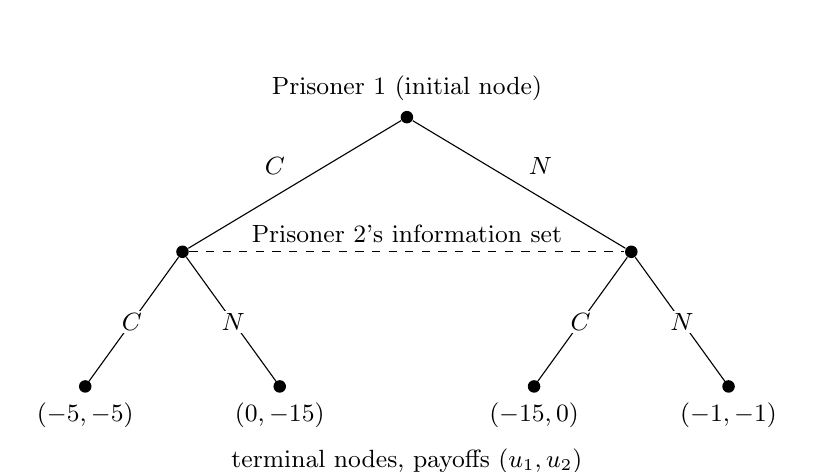
\begin{tikzpicture}[scale=0.95,
  dot/.style={circle,fill,inner sep=1.6pt}, every node/.style={font=\small}]
  \node[dot,label=above:{Prisoner 1 (initial node)}] (r) at (0,0) {};
  \node[dot] (a) at (-3,-1.8) {};
  \node[dot] (b) at (3,-1.8) {};
  \draw (r) -- node[above left] {$C$} (a);
  \draw (r) -- node[above right] {$N$} (b);
  \draw[dashed] (a) -- node[above] {Prisoner 2's information set} (b);
  \foreach \x/\p/\lab/\pay in {-4.3/a/$C$/{$(-5,-5)$}, -1.7/a/$N$/{$(0,-15)$},
                               1.7/b/$C$/{$(-15,0)$}, 4.3/b/$N$/{$(-1,-1)$}} {
    \node[dot,label=below:{\pay}] at (\x,-3.6) {};
    \draw (\p) -- node[fill=white,inner sep=1pt] {\lab} (\x,-3.6);
  }
  \node at (0,-4.6) {terminal nodes, payoffs $(u_1, u_2)$};
\end{tikzpicture}
\end{center}

\textbf{(b)} The initial node (root) is player~1's decision. The four terminal nodes carry the
payoffs. The dashed line joins player~2's two decision nodes into one \emph{information set}:
she does not know which node she is at, because she decides without observing player~1's choice.
This is how a tree represents simultaneous moves; drawing player~2 first instead gives the same
game.

\textbf{(c)} A strategy assigns an action to each information set. Player~1 has one, player~2
has one (not two), so $S_1 = S_2 = \{C, N\}$: two strategies each. Without the dashed line
player~2 would have $2^2 = 4$ strategies, as in item~3.

\textbf{Dominance and Pareto (the lecture's lessons).} For each prisoner, $C$ strictly dominates
$N$: $-5 > -15$ against $C$ and $0 > -1$ against $N$. So $(C,C)$ is the strict dominant-strategy
equilibrium, and by slide~29 the unique IESDS survivor. But $(N,N)$ gives $(-1,-1)$, better for
both than $(-5,-5)$: the equilibrium is not Pareto optimal (slides~25--26, Lessons~1 and~2).

\interp The information set encodes what a player knows when moving, and therefore what her
strategies can depend on. In the dilemma, individually rational choices waste five years each.

\verify \texttt{check\_A.py} checks that $C$ strictly dominates $N$ for both players, that
IESDS leaves only $(C,C)$, and that $(N,N)$ Pareto-dominates it. The book's answer (p.~10)
agrees on (a)--(c); the dominance paragraph goes beyond it.

\answer{Tree above: root = prisoner~1's choice, four terminal nodes with payoffs $(-5,-5)$,
$(0,-15)$, $(-15,0)$, $(-1,-1)$, and one information set joining prisoner~2's nodes because she
cannot observe prisoner~1. Each player has two strategies, $\{C, N\}$. Confess is strictly
dominant; $(C,C)$ is Pareto-dominated by $(N,N)$.}
\end{exsol}

\begin{exsol}{5}{\MG{} Ch.~1, Exercise 13}{26}{Foundations}{B2}
\asked For the $3 \times 2$ game of Fig.~1.33: (a) strictly dominant strategies; (b) strictly
dominated strategies; (c) the profiles that survive IESDS, with the steps and their
justification.

\method Definitions of strict/weak dominance and dominant strategies (Lecture~1, slide~23;
Tadelis \S4.1, pp.~59--63); IESDS as in slide~29 (Tadelis \S4.2, p.~65).

\solution
Player~1 chooses $U, M, D$; player~2 chooses $L, R$ (matrix read from the book, p.~26).
\begin{center}
\begin{tabular}{r|c|c|}
\multicolumn{1}{r}{1 $\backslash$ 2} & \multicolumn{1}{c}{$L$} & \multicolumn{1}{c}{$R$}\\ \cline{2-3}
$U$ & $-10,\ 10$ & $0,\ 12$ \\ \cline{2-3}
$M$ & $-12,\ 0$ & $2,\ 2$ \\ \cline{2-3}
$D$ & $-9,\ 0$ & $1,\ 0$ \\ \cline{2-3}
\end{tabular}
\end{center}

\textbf{(a) Dominant strategies.} Player~1: against $L$ the best row is $D$ ($-9$), against $R$
it is $M$ ($2$). A strictly dominant strategy would have to be the unique best row in every
column, so none exists. Player~2: $R$ is strictly better than $L$ in rows $U$ ($12 > 10$) and
$M$ ($2 > 0$) but equal in row $D$ ($0 = 0$). So $R$ \emph{weakly} dominates $L$ and is weakly
dominant, but not strictly. No player has a strictly dominant strategy.

\textbf{(b) Dominated strategies.} Player~1: $U$ is strictly dominated by $D$:
$u_1(U,L) = -10 < -9 = u_1(D,L)$ and $u_1(U,R) = 0 < 1 = u_1(D,R)$. $M$ is not dominated (it
is the best reply to $R$), and neither is $D$ (best reply to $L$). Player~2: $L$ is only weakly
dominated (tie in row $D$), $R$ is not dominated. The only strictly dominated strategy is $U$.

\textbf{(c) IESDS.}
\begin{itemize}
  \item Round 1: $S_1^1 = \{M, D\}$ ($U$ removed by rationality of player~1), $S_2^1 = \{L, R\}$.
  \item Round 2: in the reduced game, player~2's payoffs are $(0, 0)$ from $L$ and $(2, 0)$ from
  $R$ in rows $(M, D)$: still only weak dominance. Player~1's $M$ and $D$ remain best replies to
  $R$ and $L$ respectively. Nothing else is removed.
\end{itemize}
\[
  S^\infty = \{M, D\} \times \{L, R\} = \{(M,L), (M,R), (D,L), (D,R)\}.
\]
Why this is legitimate: a rational player~1 never plays $U$ (Lesson~1). Since rationality is
common knowledge, player~2 knows it and reasons on the reduced game; there, nothing more can be
ruled out by strict dominance.

\interp IESDS stops at four profiles because the remaining comparisons are only weak. If we
also deleted weakly dominated strategies, player~2 would drop $L$ and player~1 would then pick
$M$ (2 against 1), giving $(M,R)$. That stronger prediction depends on player~2 being sure
that player~1 never plays $D$, where the two columns tie, which is why strict elimination does
not make it (compare item~19).

\verify \texttt{check\_A.py} confirms that $U$ is strictly dominated only by $D$, that $R$
weakly but not strictly dominates $L$ (before and after round~1), and that IESDS ends after one
round with the four profiles above. The book's answer (pp.~26--28) agrees on (a), (b) and (c).

\answer{(a) None (player~2's $R$ is only weakly dominant). (b) Only $U$, strictly dominated by
$D$. (c) Delete $U$; nothing else is strictly dominated, so $S^\infty = \{M, D\} \times \{L, R\}$.}
\end{exsol}

\begin{exsol}{6}{Tadelis Exercise 4.5}{77}{Foundations}{B3}
\asked Find the strategy profiles of the given $3 \times 3$ game that survive IESDS.

\method IESDS round by round (Lecture~1, slides~28--29; Tadelis \S4.2.1, p.~65): in each round
remove every strategy that is strictly dominated given the opponent's surviving strategies.

\solution
Matrix as printed in the book (p.~77):
\begin{center}
\begin{tabular}{r|c|c|c|}
\multicolumn{1}{r}{1 $\backslash$ 2} & \multicolumn{1}{c}{$L$} & \multicolumn{1}{c}{$C$} & \multicolumn{1}{c}{$R$}\\ \cline{2-4}
$U$ & $6,\ 8$ & $2,\ 6$ & $8,\ 2$ \\ \cline{2-4}
$M$ & $8,\ 2$ & $4,\ 4$ & $9,\ 5$ \\ \cline{2-4}
$D$ & $8,\ 10$ & $4,\ 6$ & $6,\ 7$ \\ \cline{2-4}
\end{tabular}
\end{center}

\textbf{Round 1} ($S^0$ = full game).
\begin{itemize}
  \item Player~1: $U$ is strictly dominated by $M$: $6 < 8$, $2 < 4$, $8 < 9$. $D$ is not
  dominated by $M$ (ties $8 = 8$ and $4 = 4$), and $M$, $D$ are not dominated by $U$.
  \item Player~2: her payoffs are $L = (8, 2, 10)$, $C = (6, 4, 6)$, $R = (2, 5, 7)$ in rows
  $(U, M, D)$. $C$ is beaten by $L$ in rows $U, D$ but not in $M$; it beats $R$ in row $U$. No
  column is strictly dominated.
\end{itemize}
$S_1^1 = \{M, D\}$, $S_2^1 = \{L, C, R\}$.

\textbf{Round 2.} Player~2 now compares columns on rows $(M, D)$ only:
$L = (2, 10)$, $C = (4, 6)$, $R = (5, 7)$. $C$ is strictly dominated by $R$ ($4 < 5$, $6 < 7$);
$L$ and $R$ are not ranked. Player~1 on all three columns: $M = (8, 4, 9)$, $D = (8, 4, 6)$:
$M$ is better only against $R$, so $D$ is weakly but not strictly dominated.
$S_1^2 = \{M, D\}$, $S_2^2 = \{L, R\}$.

\textbf{Round 3.} Player~1 on $(L, R)$: $M = (8, 9)$, $D = (8, 6)$, a tie against $L$, so no
strict dominance. Player~2 on $(M, D)$: $L = (2, 10)$, $R = (5, 7)$, not ranked. The process
stops.
\[
  S^\infty = \{M, D\} \times \{L, R\} = \{(M,L), (M,R), (D,L), (D,R)\}.
\]

\interp Rationality of player~1 removes $U$. Then player~2's knowledge that player~1 is rational
removes $C$, which can be a best reply only to beliefs that put positive weight on $U$. The iterated-elimination
equilibrium is a set of four profiles, not a point. Two of them, $(M,R)$ with payoffs $(9,5)$
and $(D,L)$ with $(8,10)$, are profiles where each strategy is a best reply to the other (the
pure Nash equilibria of Lecture~2). Deleting the weakly dominated $D$ as well would single out
$(M,R)$, which is a stronger and less safe assumption (see item~19).

\verify \texttt{check\_A.py} runs IESDS with the lecture's definition and finds exactly the
rounds above (round~1: $U$; round~2: $C$; then stop), that $U$ is dominated only by $M$ and $C$
only by $R$, and that $D$ is weakly dominated by $M$ in the final set.

\answer{Round~1: delete $U$ (dominated by $M$). Round~2: delete $C$ (dominated by $R$ once $U$
is gone). Nothing else is strictly dominated:
$S^\infty = \{M, D\} \times \{L, R\}$, four profiles.}
\end{exsol}

\begin{exsol}{7}{Gibbons Problem 1.2}{48}{Foundations}{B3}
\asked Which strategies of the given $3 \times 3$ game survive IESDS, and what are the
pure-strategy Nash equilibria?

\method IESDS (Gibbons \S1.1.B, pp.~4--7; Lecture~1, slide~29). For the second question, a pure
Nash equilibrium is a profile in which each player's strategy is a best reply to the other's
(Gibbons \S1.1.C; Lecture~2). Every Nash equilibrium survives IESDS (Gibbons Prop.~B, p.~12), so
we only need to search the surviving cells.

\solution
The matrix as printed (the top-left cell reads ``2.0'' in the scan; it is $(2,0)$):
\begin{center}
\begin{tabular}{r|c|c|c|}
\multicolumn{1}{r}{1 $\backslash$ 2} & \multicolumn{1}{c}{$L$} & \multicolumn{1}{c}{$C$} & \multicolumn{1}{c}{$R$}\\ \cline{2-4}
$T$ & $2,\ 0$ & $1,\ 1$ & $4,\ 2$ \\ \cline{2-4}
$M$ & $3,\ 4$ & $1,\ 2$ & $2,\ 3$ \\ \cline{2-4}
$B$ & $1,\ 3$ & $0,\ 2$ & $3,\ 0$ \\ \cline{2-4}
\end{tabular}
\end{center}

\textbf{Round 1.} Player~1: $B$ is strictly dominated by $T$ ($1 < 2$, $0 < 1$, $3 < 4$); it is
not dominated by $M$ ($3 > 2$ against $R$). $T$ and $M$ are best replies to $R$ and $L$, so they
stay. Player~2, columns over rows $(T, M, B)$: $L = (0, 4, 3)$, $C = (1, 2, 2)$, $R = (2, 3, 0)$.
$C$ is \emph{not} dominated yet: it beats $R$ in row $B$ ($2 > 0$) and $L$ in row $T$.
$S_1^1 = \{T, M\}$, $S_2^1 = \{L, C, R\}$.

\textbf{Round 2.} On rows $(T, M)$: $C = (1, 2)$ and $R = (2, 3)$, so $C$ is strictly dominated by
$R$. $L = (0, 4)$ and $R = (2, 3)$ are not ranked. $S_2^2 = \{L, R\}$.

\textbf{Round 3.} Player~1 on $(L, R)$: $T = (2, 4)$, $M = (3, 2)$, not ranked. Player~2 on
$(T, M)$: $L = (0, 4)$, $R = (2, 3)$, not ranked. Stop.
\[
  S^\infty = \{T, M\} \times \{L, R\}.
\]

\textbf{Pure Nash equilibria.} Check the four surviving cells:
\begin{itemize}
  \item $(T, L)$: player~1 would switch to $M$ ($3 > 2$). Not NE.
  \item $(T, R)$: player~1 gets $4 \ge 3, 2$ in column $R$; player~2 gets $2 \ge 0, 1$ in row $T$. NE.
  \item $(M, L)$: player~1 gets $3 \ge 2, 1$; player~2 gets $4 \ge 2, 3$. NE.
  \item $(M, R)$: player~1 would switch to $T$ ($4 > 2$). Not NE.
\end{itemize}
The pure Nash equilibria are $(T, R)$ and $(M, L)$.

\interp Note the order: $C$ is a sensible reply only to beliefs that put weight on $B$; once
player~2 knows player~1 is rational, $C$ goes. IESDS leaves four profiles; Nash equilibrium,
which requires beliefs to be correct, cuts them to two. This previews Lecture~2.

\verify \texttt{check\_A.py} reproduces the rounds (round~1: $B$; round~2: $C$), checks that $C$
is not dominated in the full game, and finds by brute force over all nine cells that the pure
Nash equilibria are exactly $(T,R)$ and $(M,L)$. Kumar's unofficial Gibbons manual (Answer~1.2,
not in \texttt{Livros/}) gives the same deletions and equilibria; it writes the survivors as
``(T,M) and (L,R)'', meaning $\{T,M\}$ for player~1 and $\{L,R\}$ for player~2.

\answer{IESDS: delete $B$ (by $T$), then $C$ (by $R$); survivors $\{T, M\} \times \{L, R\}$.
Pure Nash equilibria: $(T, R)$ with payoffs $(4,2)$ and $(M, L)$ with payoffs $(3,4)$.}
\end{exsol}

\begin{exsol}{8}{\MG{} Ch.~1, Exercise 9}{17}{Foundations}{B3}
\asked Apply IESDS to the husband--wife Battle of the Sexes of Fig.~1.22 (p.~18) and state the
most precise prediction it gives.

\method IESDS (Lecture~1, slide~29); evaluation criteria for solution concepts, in particular
uniqueness (slide~22; Tadelis \S4.2.3, pp.~67--68).

\solution
\begin{center}
\begin{tabular}{r|c|c|}
\multicolumn{1}{r}{Husband $\backslash$ Wife} & \multicolumn{1}{c}{$F$} & \multicolumn{1}{c}{$O$}\\ \cline{2-3}
$F$ & $3,\ 1$ & $0,\ 0$ \\ \cline{2-3}
$O$ & $0,\ 0$ & $1,\ 3$ \\ \cline{2-3}
\end{tabular}
\end{center}
\begin{itemize}
  \item Husband: $u_H(F,F) = 3 > 0 = u_H(O,F)$ but $u_H(O,O) = 1 > 0 = u_H(F,O)$. Each strategy
  is strictly better against one of the wife's strategies, so neither is dominated, strictly
  or weakly.
  \item Wife: $u_W(F,F) = 1 > 0 = u_W(F,O)$ but $u_W(O,O) = 3 > 0 = u_W(O,F)$. The same holds.
\end{itemize}
Round~1 removes nothing, so the process stops at once: $S_i^1 = S_i^0$ and
\[
  S^\infty = \{F, O\} \times \{F, O\} = \{(F,F), (F,O), (O,F), (O,O)\}.
\]

\interp IESDS has no bite here: every profile is an iterated-elimination equilibrium,
including the miscoordinated $(F,O)$ and $(O,F)$, which no one wants. The reason is
structural. In a coordination game each strategy is the best reply to \emph{something}, so
rationality and common knowledge of rationality cannot rule anything out. IESDS exists for every
game, but it often fails on uniqueness (slide~22). What is missing is a theory of what each
player \emph{expects} the other to do. Nash equilibrium supplies it (Lecture~2) and selects
$(F,F)$ and $(O,O)$ in pure strategies. The same failure occurs in the stag hunt (item~2) and in
matching pennies (item~1).

\verify \texttt{check\_A.py} confirms that no strategy is strictly or weakly dominated and
that IESDS returns the full game. The book's answer (p.~18) agrees: no strictly (or weakly)
dominated strategies and all four profiles survive.

\answer{No strategy is dominated for either player (each is the strict best reply to one of
the other's choices), so IESDS deletes nothing and all four profiles survive. The ``most precise
prediction'' is that anything can happen; IESDS has no bite in coordination games.}
\end{exsol}


\part*{Tier 2 --- Exam level}
\addcontentsline{toc}{part}{Tier 2 --- Exam level}
\begin{exsol}{9}{Tadelis Exercise 3.6}{58}{Exam}{B1}
\asked Write the normal form of a price game between two zero-cost firms facing demand
$p = 100 - q$, where the cheaper firm takes the whole market and equal prices split it.

\method Normal form with continuous strategy sets and piecewise payoffs, built like Tadelis's
Cournot example (\S3.1.2, p.~49) and the lecture's definition (slides~13--14, 18).

\solution
Inverting the demand curve, a firm that serves the market at price $p$ sells
$D(p) = \max\{0,\, 100 - p\}$ (no one buys at $p \ge 100$). Costs are zero, so revenue is profit.
\begin{itemize}
  \item Players: $I = \{1, 2\}$.
  \item Strategy sets: $S_i = [0, \infty)$, prices (one may cap them at $100$ without loss,
  since higher prices sell nothing).
  \item Payoffs: for $i \ne j$,
  \[
    u_i(p_i, p_j) =
    \begin{cases}
      p_i \max\{0, 100 - p_i\} & \text{if } p_i < p_j,\\[2pt]
      \tfrac12\, p_i \max\{0, 100 - p_i\} & \text{if } p_i = p_j,\\[2pt]
      0 & \text{if } p_i > p_j.
    \end{cases}
  \]
\end{itemize}
This triple $G = (\{1,2\}, \{[0,\infty)\}_{i}, \{u_i\}_{i})$ is the normal form. It cannot be
drawn as a finite matrix: each player has a continuum of strategies, and the payoff jumps at
$p_i = p_j$.

\textbf{Dominance (beyond the question).} Against $p_j = 0$ every price earns $0$ (a higher
price sells nothing; a tie at $0$ earns nothing). So no price is \emph{strictly} better than
another against every $p_j$: no strategy is strictly dominated and IESDS has no bite. Weak
dominance does bite. The monopoly price maximizes $p(100 - p)$ at $p^m = 50$
($100 - 2p = 0$), and $p^m$ earns at least as much as any $p_i \ge 100$ (which always earns 0)
or $p_i = 0$, and strictly more against $p_j > 50$. Lecture~2's Bertrand equilibrium,
$p_1 = p_2 = 0$, will therefore use weakly dominated strategies.

\interp Even a simple pricing story gives a discontinuous payoff function: undercutting by
a cent doubles the quantity sold. That discontinuity drives the Bertrand result
(Lecture~2). It is also why the normal form must specify the tie-breaking rule.

\verify \texttt{check\_B.py} builds the payoff on an integer price grid $0, \dots, 120$,
confirms that every price earns 0 against $p_j = 0$, that grid IESDS deletes nothing, that
$p = 50$ weakly dominates $p = 0$ and every $p \ge 100$, and that $50$ solves the first-order
condition (sympy).

\answer{$I = \{1,2\}$, $S_i = [0, \infty)$, and $u_i(p_i, p_j) = p_i \max\{0, 100 - p_i\}$ if
$p_i < p_j$, half of that if $p_i = p_j$, and $0$ if $p_i > p_j$. No strategy is strictly
dominated; prices $0$ and $\ge 100$ are weakly dominated by $50$.}
\end{exsol}

\begin{exsol}{10}{Tadelis Exercise 3.7}{58}{Exam}{B1}
\asked Write the normal form of the three-player streetlamp game (contribute 1 or nothing; the
lamp, worth 3 to everyone, is built iff at least two contribute; contributions are not
refunded).

\method Normal form with $n = 3$ players (slides~13--14); a three-player game is drawn as one
matrix for players~1 and~2 per strategy of player~3 (Tadelis \S3.1).

\solution
Let $s_i = 1$ if player~$i$ contributes and $s_i = 0$ otherwise.
\begin{itemize}
  \item Players: $I = \{1, 2, 3\}$; strategies $S_i = \{0, 1\}$, so $|S| = 2^3 = 8$ profiles.
  \item Payoffs: the lamp is built iff $s_1 + s_2 + s_3 \ge 2$, so
  \[
    u_i(s_1, s_2, s_3) = 3 \cdot \mathbf{1}\{s_1 + s_2 + s_3 \ge 2\} - s_i .
  \]
\end{itemize}
Payoffs $(u_1, u_2, u_3)$; player~1 picks the row, player~2 the column, player~3 the matrix:
\begin{center}
\begin{tabular}{r|c|c|}
\multicolumn{3}{c}{Player 3: $s_3 = 0$}\\
\multicolumn{1}{r}{1 $\backslash$ 2} & \multicolumn{1}{c}{$0$} & \multicolumn{1}{c}{$1$}\\ \cline{2-3}
$0$ & $0,\ 0,\ 0$ & $0,\ -1,\ 0$ \\ \cline{2-3}
$1$ & $-1,\ 0,\ 0$ & $2,\ 2,\ 3$ \\ \cline{2-3}
\end{tabular}
\qquad
\begin{tabular}{r|c|c|}
\multicolumn{3}{c}{Player 3: $s_3 = 1$}\\
\multicolumn{1}{r}{1 $\backslash$ 2} & \multicolumn{1}{c}{$0$} & \multicolumn{1}{c}{$1$}\\ \cline{2-3}
$0$ & $0,\ 0,\ -1$ & $3,\ 2,\ 2$ \\ \cline{2-3}
$1$ & $2,\ 3,\ 2$ & $2,\ 2,\ 2$ \\ \cline{2-3}
\end{tabular}
\end{center}

\textbf{Dominance (beyond the question).} Player~$i$'s best action depends on how many
\emph{others} contribute, $m \in \{0, 1, 2\}$:
\[
  u_i(1; m) - u_i(0; m) = \begin{cases} -1 & m = 0 \text{ (lamp fails either way)},\\
  3 - 1 = 2 & m = 1 \text{ (player $i$ is pivotal)},\\ -1 & m = 2 \text{ (lamp built anyway)}.\end{cases}
\]
Neither action is dominated, so IESDS removes nothing. The profiles where every player is
best-replying are ``nobody contributes'' and the three profiles with exactly two contributors.

\interp Contributing pays only when one is pivotal. That is the free-rider problem of public
goods: with two others contributing, a player keeps her coin. The game has both
coordination (no lamp vs.\ lamp) and conflict (who pays).

\verify \texttt{check\_A.py} evaluates the payoff formula on all eight profiles (it matches the
matrices), confirms that IESDS deletes nothing for any player, and finds the four profiles with
mutual best replies by brute force.

\answer{$I = \{1,2,3\}$, $S_i = \{0,1\}$, $u_i(s) = 3\cdot\mathbf{1}\{\sum_j s_j \ge 2\} - s_i$;
matrices above, one per choice of player~3. No strategy is dominated: contributing pays iff
exactly one other player contributes.}
\end{exsol}

\begin{exsol}{11}{Tadelis Exercise 4.1}{76}{Exam}{B2}
\asked Prove Tadelis's Proposition~4.1 (p.~61): a strict dominant-strategy equilibrium, if it
exists, is the unique dominant-strategy equilibrium.

\method Direct proof by contradiction from the definitions (Lecture~1, slides~23 and~25;
Tadelis Defs.~4.1--4.3, pp.~60--61). ``Dominant-strategy equilibrium'' is read in the widest
sense: a profile in which every player uses a dominant strategy, strict \emph{or} weak.
Tadelis defines weak dominance with ``$\ge$ for all $\sm$'' (Remark, p.~63); the lecture adds
``$>$ for some $\sm$''. The proof works under both readings because it only uses the ``$\ge$''
part.

\solution
\textbf{Claim.} Let $s^D \in S$ be a strict dominant-strategy equilibrium of
$G = (I, \{S_i\}, \{u_i\})$: for every $i \in I$,
\[
  u_i(s_i^D, \sm) > u_i(s_i', \sm) \qquad \forall s_i' \in S_i \setminus \{s_i^D\},\ \forall \sm \in \Sm. \tag{1}
\]
If $s^W \in S$ is a profile in which every player uses a (strictly or weakly) dominant strategy,
then $s^W = s^D$.

\textbf{Proof.} Suppose not. Then there is a player $i$ with $s_i^W \ne s_i^D$. Because $s_i^W$ is
(at least weakly) dominant, it does at least as well as every strategy, in particular $s_i^D$:
\[
  u_i(s_i^W, \sm) \ge u_i(s_i^D, \sm) \qquad \forall \sm \in \Sm. \tag{2}
\]
Take any $\sm \in \Sm$ (the set is nonempty). Applying (1) with $s_i' = s_i^W$ gives
$u_i(s_i^D, \sm) > u_i(s_i^W, \sm)$, which contradicts (2) at that $\sm$. Hence $s_i^W = s_i^D$
for every $i$, that is, $s^W = s^D$. \hfill$\square$

\textbf{What the proof uses.} Only the definitions; no finiteness. Two by-products:
\begin{enumerate}[label=(\roman*)]
  \item A player has at most one strictly dominant strategy (take $s^W_i$ strictly dominant
  in the argument).
  \item If the dominance were only weak in (1), the argument fails: two strategies can each be
  ``$\ge$'' the other everywhere when they tie everywhere. That is exactly Exercise~4.2(b)
  (item~12).
\end{enumerate}
The lecture's other proposition (slide~29; Tadelis Prop.~4.2, p.~68) adds that $s^D$ is also the
unique IESDS survivor: in round~1 every $s_i' \ne s_i^D$ is strictly dominated by $s_i^D$.

\interp When it exists, strict dominance gives a unique prediction and asks very little of the
players (only their own rationality). The cost is existence: most games have no strictly dominant
strategies (item~8).

\verify \texttt{check\_C.py} draws 20\,000 random games ($2\times2$, $2\times3$, $3\times2$,
payoffs in $\{0,\dots,4\}$). Whenever both players have a strictly dominant strategy, it checks
that the strictly dominant strategy is the only ``$\ge$-dominant'' one for each player and the
only IESDS survivor.

\answer{If $s_i^W \ne s_i^D$ for some $i$, weak dominance of $s_i^W$ gives
$u_i(s_i^W, \sm) \ge u_i(s_i^D, \sm)$ for all $\sm$, while strict dominance of $s_i^D$ gives the
reverse strict inequality, a contradiction. So any dominant-strategy equilibrium equals $s^D$.}
\end{exsol}

\begin{exsol}{12}{Tadelis Exercise 4.2}{76}{Exam}{B2}
\asked Using Tadelis's definition of a weakly dominant strategy equilibrium, give (a) a game
with no such equilibrium and (b) a game with more than one.

\method Definitions. Tadelis calls $s_i^W$ weakly dominant if
$u_i(s_i^W, \sm) \ge u_i(s_i', \sm)$ for all $s_i'$ and all $\sm$, with no strictness required
(statement of 4.2 and Remark, p.~63). The lecture's weak dominance (slide~23) also asks for a
strict inequality at some $\sm$. Which definition is used matters for (b).

\solution
\textbf{(a) No weakly dominant strategy equilibrium.} Matching pennies (Tadelis 3.5), or the
penalty kicks of item~1:
\begin{center}
\begin{tabular}{r|c|c|}
\multicolumn{1}{r}{1 $\backslash$ 2} & \multicolumn{1}{c}{$H$} & \multicolumn{1}{c}{$T$}\\ \cline{2-3}
$H$ & $1,\ -1$ & $-1,\ 1$ \\ \cline{2-3}
$T$ & $-1,\ 1$ & $1,\ -1$ \\ \cline{2-3}
\end{tabular}
\end{center}
For player~1, $H$ does worse than $T$ against $T$ ($-1 < 1$), and $T$ does worse than $H$ against
$H$. So neither satisfies ``$\ge$ every other strategy for every $s_2$''. The same holds for
player~2. No player has a weakly dominant strategy, so there is no weakly dominant strategy
equilibrium. (The Battle of the Sexes, item~8, works too.)

\textbf{(b) More than one.} Make one player indifferent between two strategies and give the
other a dominant strategy:
\begin{center}
\begin{tabular}{r|c|c|}
\multicolumn{1}{r}{1 $\backslash$ 2} & \multicolumn{1}{c}{$L$} & \multicolumn{1}{c}{$R$}\\ \cline{2-3}
$U$ & $2,\ 3$ & $0,\ 1$ \\ \cline{2-3}
$D$ & $2,\ 1$ & $0,\ 0$ \\ \cline{2-3}
\end{tabular}
\end{center}
Player~1's payoffs from $U$ and $D$ coincide column by column ($2 = 2$, $0 = 0$), so each
satisfies Tadelis's ``$\ge$'' condition against the other: both are weakly dominant. For
player~2, $L$ strictly dominates $R$ ($3 > 1$, $1 > 0$). Hence $(U, L)$ and $(D, L)$ are both
weakly dominant strategy equilibria. They are not equivalent: player~2 gets $3$ in one and $1$
in the other. This is the same idea as the MWG solutions manual's example for MWG
Exercise~8.B.2(b).

\textbf{The role of the definition.} Under the lecture's definition, (b) is impossible. If
$s_i$ and $s_i'$ were both weakly dominant, $s_i$ would weakly dominate $s_i'$, so
$u_i(s_i, \sm) > u_i(s_i', \sm)$ for some $\sm$, while $s_i'$ weakly dominating $s_i$ requires
$u_i(s_i', \sm) \ge u_i(s_i, \sm)$ at that same $\sm$. Contradiction. So each player has at most
one weakly dominant strategy and there is at most one weakly dominant-strategy equilibrium. In
general, as MWG Exercise~8.B.2(a) shows, two strategies that are both weakly dominant in the
``$\ge$'' sense give equal payoffs against every $\sm$. Multiplicity comes only from such ties.

\interp Weak dominance is a weaker requirement, so an equilibrium in weakly dominant
strategies is easier to have (the second-price auction, item~23) but need not be unique. The
non-uniqueness here is harmless for the indifferent player but not for the other one.

\verify \texttt{check\_C.py} checks that no strategy in matching pennies is ``$\ge$-dominant'',
that $U$ and $D$ are both ``$\ge$-dominant'' and $L$ strictly dominant in the example, that player~2
prefers $(U,L)$, and, on 20\,000 random games, that under the lecture's definition no player ever
has two weakly dominant strategies.

\answer{(a) Matching pennies: every strategy is strictly worse than the other against some
opponent strategy, so no weakly dominant strategy exists. (b) In the $2\times2$ game above,
$U$ and $D$ tie for player~1 and $L$ is strictly dominant for player~2, so $(U,L)$ and $(D,L)$
are both weakly dominant strategy equilibria. (b) needs Tadelis's ``$\ge$ only'' definition;
under the lecture's definition it cannot happen.}
\end{exsol}

\begin{exsol}{13}{MWG Exercise 8.B.1}{262}{Exam}{B2}
\asked $I$ firms choose lobbying hours $h_i \ge 0$ at cost $w_i h_i^2$; the subsidy is worth
$\alpha \sum_i h_i + \beta \prod_i h_i$. Show that each firm has a strictly dominant strategy if
and only if $\beta = 0$, and find it.

\method Strict dominance (MWG Def.~8.B.1, p.~237; Lecture~1, slide~23) in a game with
continuous strategies. With a strictly concave payoff, the best reply is unique. So a strategy
is strictly dominant exactly when it is the best reply to \emph{every} profile of the others.

\solution
We take firm~$i$'s payoff to be the value of the subsidy minus its own cost (as the MWG
solutions manual does), with $I \ge 2$, $w_i > 0$. Write $P_{-i} = \prod_{j\ne i} h_j \ge 0$:
\[
  u_i(h_i, h_{-i}) = (\alpha + \beta P_{-i})\, h_i - w_i h_i^2 + \alpha \textstyle\sum_{j\ne i} h_j .
\]
The last term does not depend on $h_i$. Also $\partial^2 u_i/\partial h_i^2 = -2w_i < 0$.

\textbf{Step 1: best reply.} Strict concavity on $[0, \infty)$ gives the unique maximizer
\[
  BR_i(h_{-i}) = \max\Big\{0,\ \frac{\alpha + \beta P_{-i}}{2 w_i}\Big\}.
\]
When positive, it solves the first-order condition $\alpha + \beta P_{-i} - 2 w_i h_i = 0$.

\textbf{Step 2: dominance $\Leftrightarrow$ constant best reply.} If $h_i^*$ is strictly dominant,
it is a best reply to every $h_{-i}$, so $BR_i$ is the constant $h_i^*$. Conversely, if
$BR_i(h_{-i}) = h_i^*$ for all $h_{-i}$, uniqueness of the maximizer gives
$u_i(h_i^*, h_{-i}) > u_i(h_i, h_{-i})$ for every $h_i \ne h_i^*$ and every $h_{-i}$: $h_i^*$ is
strictly dominant. With $I \ge 2$, $P_{-i}$ takes every value in $[0,\infty)$ (set each
$h_j = P^{1/(I-1)}$).

\textbf{Step 3: when is $BR_i$ constant in $P_{-i} \in [0, \infty)$?}
\begin{itemize}
  \item $\beta = 0$: $BR_i = \max\{0, \alpha/(2w_i)\}$, constant. \emph{Dominant.} For $\alpha > 0$,
  \[
    u_i(h_i^*, h_{-i}) - u_i(h_i, h_{-i}) = w_i\,(h_i - h_i^*)^2 > 0 \quad (h_i \ne h_i^*),
    \qquad h_i^* = \frac{\alpha}{2 w_i}.
  \]
  \item $\beta > 0$: $(\alpha + \beta P)/(2w_i) \to \infty$ as $P \to \infty$. Not constant: no
  dominant strategy (more effort by others raises the return to own effort).
  \item $\beta < 0$, $\alpha > 0$: $BR_i = \alpha/(2w_i) > 0$ at $P = 0$ but $BR_i = 0$ for
  $P \ge \alpha/|\beta|$. Not constant.
  \item $\beta < 0$, $\alpha \le 0$: $\alpha + \beta P \le 0$ for all $P \ge 0$, so $BR_i \equiv 0$.
  \emph{Dominant}, although $\beta \ne 0$: for $h_i > 0$,
  $u_i(0, h_{-i}) - u_i(h_i, h_{-i}) = -(\alpha + \beta P_{-i}) h_i + w_i h_i^2 > 0$.
\end{itemize}
So ``strictly dominant $\Leftrightarrow \beta = 0$'' holds whenever $\alpha > 0$, the case in
which lobbying is productive and the dominant strategy is interior. At the corner, when
$\alpha \le 0$ and $\beta < 0$, lobbying never pays, so $h_i = 0$ is strictly dominant for any
such $\beta$.

\interp $\beta \ne 0$ makes efforts interact: with $\beta > 0$ they are complements (others'
hours raise my marginal return), so my best choice depends on what I expect them to do and no
strategy is dominant. With $\beta = 0$ each firm's problem is separable: it equates its own
marginal benefit $\alpha$ to its marginal cost $2w_i h_i$, whatever the others do. Even then the
outcome is not efficient for the industry: each firm ignores that its hours also benefit the
other firms' subsidy, the same wedge as in the prisoner's dilemma (slide~26).

\verify \texttt{check\_B.py} derives the best reply and the second derivative with sympy, checks
the identity $u_i(h^*) - u_i(h) = w_i(h - h^*)^2$ for $\beta = 0$, and tests nine sign
combinations of $(\alpha, \beta)$ on values of $P_{-i}$ from 0 to $10^3$: the best reply is
constant exactly when $\beta = 0$ or ($\beta < 0$, $\alpha \le 0$). \emph{Comparison with the MWG
solutions manual} (p.~8-1): it agrees on the first-order condition, the ``iff $\beta = 0$'' and
$h_i = \alpha/(2w_i)$, but it ignores the constraint $h_i \ge 0$. Its ``only if'' therefore
misses the corner case $\alpha \le 0$, $\beta < 0$, and for $\alpha < 0$, $\beta = 0$ its formula
gives a negative number of hours (the dominant strategy is then $h_i = 0$).

\answer{Each firm's payoff is strictly concave with best reply
$\max\{0, (\alpha + \beta\prod_{j\ne i}h_j)/(2w_i)\}$, and a strategy is strictly dominant iff
this best reply is constant. For $\alpha > 0$ that happens iff $\beta = 0$, and the strictly
dominant strategy is $h_i^* = \alpha/(2w_i)$. (Corner: with $\alpha \le 0$ the dominant strategy
is $h_i = 0$, also when $\beta < 0$.)}
\end{exsol}

\begin{exsol}{14}{\MG{} Ch.~1, Exercise 12}{23}{Exam}{B3}
\asked For the $3 \times 3$ game of Fig.~1.30: (a) strictly dominant strategies; (b) strictly
dominated strategies; (c) what each player deletes under rationality alone; (d) what survives
under common knowledge of rationality (IESDS).

\method Dominance (slide~23) and the epistemic reading of IESDS (slide~28; Tadelis \S4.2.1,
p.~65). Round~1 of IESDS uses only each player's own rationality. Round~2 uses ``each knows the
other is rational'', and so on.

\solution
Matrix from the book (p.~23):
\begin{center}
\begin{tabular}{r|c|c|c|}
\multicolumn{1}{r}{1 $\backslash$ 2} & \multicolumn{1}{c}{$F$} & \multicolumn{1}{c}{$C$} & \multicolumn{1}{c}{$B$}\\ \cline{2-4}
$F$ & $0,\ 5$ & $2,\ 4$ & $2,\ 3$ \\ \cline{2-4}
$C$ & $2,\ 3$ & $0,\ 5$ & $3,\ 2$ \\ \cline{2-4}
$B$ & $5,\ 0$ & $2,\ 4$ & $2,\ 3$ \\ \cline{2-4}
\end{tabular}
\end{center}

\textbf{(a)} Player~1's best rows are $B$ against $F$ (5), $F$ or $B$ against $C$ (tie at 2),
and $C$ against $B$ (3). No row is the unique best everywhere: no strictly dominant strategy.
Player~2's best columns are $F$ in row $F$ (5), $C$ in row $C$ (5), $C$ in row $B$ (4): none is
best everywhere. Neither player has a strictly dominant strategy.

\textbf{(b)} Player~1: $F = (0, 2, 2)$, $C = (2, 0, 3)$, $B = (5, 2, 2)$ over columns
$(F, C, B)$. $B$ and $C$ are the unique best replies to columns $F$ and $B$, so they are not
dominated; $F$ ties with $B$ against columns $C$ and $B$ and beats $C$ against column $C$, so it
is not strictly dominated either (it is weakly dominated by $B$). No row is strictly dominated. Player~2:
$F = (5, 3, 0)$, $C = (4, 5, 4)$, $B = (3, 2, 3)$ over rows $(F, C, B)$. $B$ is strictly dominated
by $C$: $3 < 4$, $2 < 5$, $3 < 4$. $F$ and $C$ are not dominated (each is the best reply to some
row). The only strictly dominated strategy is player~2's $B$.

\textbf{(c) Rationality, no common knowledge.} Each player deletes his own strictly dominated
strategies but does not use the fact that the other does the same. Player~2 drops $B$;
player~1 has nothing to drop and still evaluates his rows against all three columns:
\[
  \{F, C, B\} \times \{F, C\} = \{(F,F), (F,C), (C,F), (C,C), (B,F), (B,C)\}.
\]

\textbf{(d) Common knowledge of rationality.} Player~1 knows player~2 is rational, so he compares
rows on columns $\{F, C\}$ only: $F = (0, 2)$, $C = (2, 0)$, $B = (5, 2)$. Now $C$ is strictly
dominated by $B$ ($2 < 5$, $0 < 2$); $F$ is only weakly dominated by $B$ (tie against $C$).
Round~3: player~2 compares $F = (5, 0)$ and $C = (4, 4)$ on rows $(F, B)$; neither dominates.
Player~1 compares $F = (0, 2)$ and $B = (5, 2)$; only weak. Stop:
\[
  S^\infty = \{F, B\} \times \{F, C\} = \{(F,F), (F,C), (B,F), (B,C)\}.
\]

\interp Rationality alone removes only strategies that are bad against \emph{everything}.
Player~1's $C$ is a good reply to $B$, so it can only be discarded by someone who knows that
player~2 will not play $B$, that is, by someone who uses player~2's rationality. Each extra layer
of ``I know that you know'' can remove more strategies; here two layers suffice.

\verify \texttt{check\_A.py} checks the dominance statements in (a)--(b), that IESDS removes $B$
for player~2 in round~1 and $C$ for player~1 in round~2, and that $F$ is only weakly dominated
by $B$ in the final game. The book's answer (pp.~23--26) agrees with (a)--(d). Its text for (b)
and (d) describes the comparisons loosely (for example, it says player~1 deletes $C$ because his
payoff ``is higher from $B$ \dots when player 2 plays $F$''), but the deletions and the final
sets are the same as ours.

\answer{(a) None. (b) Only player~2's $B$ (strictly dominated by $C$). (c) Rationality alone:
$\{F, C, B\} \times \{F, C\}$, six profiles. (d) With common knowledge, player~1 then drops $C$
(dominated by $B$ on $\{F, C\}$): $S^\infty = \{F, B\} \times \{F, C\}$, four profiles.}
\end{exsol}

\begin{exsol}{15}{Tadelis Exercise 4.6}{77}{Exam}{B3}
\asked Two roommates choose cleaning times $t_i \ge 0$ with payoff
$u_i = (10 - t_j)\,t_i - t_i^2$. Find (a) the best-response correspondence, (b) the choices that
survive one round of IESDS, and (c) those that survive IESDS.

\method IESDS with continuous strategies by bounding best replies, exactly as in Tadelis's
Cournot example (\S4.2.2, pp.~65--67, Fig.~4.1). Tool: for a payoff that is a concave parabola
in own action, an action outside the range of possible best replies is strictly dominated by the
nearest end of that range.

\solution
\textbf{(a) Best response.} $u_i$ is strictly concave in $t_i$ ($\partial^2 u_i/\partial t_i^2 = -2$).
The first-order condition $10 - t_j - 2t_i = 0$ and the constraint $t_i \ge 0$ give the unique
best reply
\[
  BR_i(t_j) = \max\Big\{0,\ \frac{10 - t_j}{2}\Big\} = \max\Big\{0,\ 5 - \frac{t_j}{2}\Big\}.
\]
It is a function (single-valued) and decreasing in $t_j$: cleaning is a strategic substitute.

\textbf{Dominance lemma.} Write $x = (10 - t_j)/2$, so $u_i(t, t_j) = t(2x - t)$. For any two
times $a, t$,
\[
  u_i(a, t_j) - u_i(t, t_j) = (t - a)\,(t + a - 2x). \tag{1}
\]
If $t > a \ge x$ the right side is positive; if $t < a \le x$ it is positive too. So if every
possible $x$ (given the opponent's surviving set) lies in $[\underline{a}, \bar a]$, then every
$t > \bar a$ is strictly dominated by $\bar a$ and every $t < \underline{a}$ by $\underline{a}$.
Conversely, a $t$ that is the unique best reply to some surviving $t_j$ is not strictly
dominated.

\textbf{(b) One round.} With $t_j \in [0, \infty)$, the best reply ranges over $[0, 5]$
($BR = 5$ at $t_j = 0$, $BR = 0$ for $t_j \ge 10$). By (1) with $\bar a = 5$, every $t_i > 5$
is strictly dominated by $t_i = 5$. Every $t_i \in [0,5]$ is the best reply to
$t_j = 10 - 2t_i \in [0, 10]$, so it survives. Hence $S_i^1 = [0, 5]$.

\textbf{(c) Iterating.} If $S_j^k = [L_k, U_k]$, the surviving best replies form
$[BR(U_k), BR(L_k)]$, so
\[
  L_{k+1} = 5 - \tfrac{U_k}{2}, \qquad U_{k+1} = 5 - \tfrac{L_k}{2}, \qquad (L_1, U_1) = (0, 5).
\]
\begin{center}
\begin{tabular}{c|cccccc}
$k$ & 1 & 2 & 3 & 4 & 5 & $\infty$ \\ \hline
$S_i^k$ & $[0, 5]$ & $[2.5, 5]$ & $[2.5, 3.75]$ & $[3.125, 3.75]$ & $[3.125, 3.4375]$ & $\{10/3\}$
\end{tabular}
\end{center}
The width halves each round: $U_{k+1} - L_{k+1} = \tfrac12 (U_k - L_k)$, so
$U_k - L_k = 5/2^{k-1} \to 0$. The midpoint $M_k$ satisfies $M_{k+1} = 5 - M_k/2$, whose fixed
point is $10/3$, and
\[
  M_k - \tfrac{10}{3} = \big(-\tfrac12\big)^{k-1}\big(M_1 - \tfrac{10}{3}\big)
  = \big(-\tfrac12\big)^{k-1}\big(-\tfrac56\big) \to 0 .
\]
Therefore $S_i^\infty = \bigcap_k S_i^k = \{10/3\}$ for both roommates: IESDS predicts the
unique profile $t_1 = t_2 = 10/3$, the point where $t = 5 - t/2$.

\interp Each round uses one more layer of knowledge: round~1, ``I am rational'' (never clean more
than 5 hours); round~2, ``I know you are rational'' (you clean at most 5, so I clean at least
2.5); and so on. Each player gets $u_i = (10 - 10/3)(10/3) - (10/3)^2 = 100/9$. Both cleaning
$t = 2.5$ would give $(7.5)(2.5) - 6.25 = 12.5 > 100/9$: the IESDS outcome over-cleans relative to
the joint optimum. Each roommate ignores that his cleaning lowers the value of the other's.

\verify \texttt{check\_B.py} checks the best reply and the factorization (1) with sympy, runs the
interval recursion for 40 rounds in exact arithmetic (width $5/2^{k-1}$ and the midpoint formula
at every round), and, as a second route, runs brute-force IESDS on the grid
$\{0, \tfrac16, \dots, 10\}$, which leaves exactly $t_1 = t_2 = 10/3$.

\answer{(a) $BR_i(t_j) = \max\{0, (10 - t_j)/2\}$. (b) $S_i^1 = [0, 5]$: any $t_i > 5$ is
strictly dominated by $5$. (c) Rounds give $[2.5, 5]$, $[2.5, 3.75]$, $[3.125, 3.75]$, \dots,
with widths $5/2^{k-1}$; only $t_1 = t_2 = 10/3$ survives IESDS.}
\end{exsol}

\begin{exsol}{16}{Tadelis Exercise 4.7}{77--78}{Exam}{B3}
\asked Two candidates choose a positive ($P$), balanced ($B$) or negative ($N$) campaign; payoffs
are win probabilities given by the book's rules. (a) Model it as a normal-form game; (b) write
the matrix; (c) describe each stage of IESDS and say whether it gives a clear prediction.

\method Normal form (slides~13--14); IESDS (slide~29; Tadelis \S4.2).

\solution
\textbf{(a)} $I = \{1, 2\}$, $S_1 = S_2 = \{P, B, N\}$. Let $\pi(s_i, s_j)$ be the probability that
the candidate playing $s_i$ wins against $s_j$. The book's rules give
\[
  \pi(s,s) = 0.5,\quad \pi(P,B) = 0,\quad \pi(P,N) = 0.3,\quad \pi(N,B) = 0.6 .
\]
The other three entries follow because exactly one candidate wins:
$\pi(B,P) = 1$, $\pi(N,P) = 0.7$, $\pi(B,N) = 0.4$. Payoffs are $u_1(s_1,s_2) = \pi(s_1,s_2)$ and
$u_2(s_1,s_2) = 1 - u_1(s_1,s_2) = \pi(s_2,s_1)$. Player~2's payoff function is the same rule
applied with the roles swapped. It is the complement of player~1's because the probabilities of
the two candidates winning add up to one: the game is constant-sum and symmetric.

\textbf{(b)}
\begin{center}
\begin{tabular}{r|c|c|c|}
\multicolumn{1}{r}{1 $\backslash$ 2} & \multicolumn{1}{c}{$P$} & \multicolumn{1}{c}{$B$} & \multicolumn{1}{c}{$N$}\\ \cline{2-4}
$P$ & $0.5,\ 0.5$ & $0,\ 1$ & $0.3,\ 0.7$ \\ \cline{2-4}
$B$ & $1,\ 0$ & $0.5,\ 0.5$ & $0.4,\ 0.6$ \\ \cline{2-4}
$N$ & $0.7,\ 0.3$ & $0.6,\ 0.4$ & $0.5,\ 0.5$ \\ \cline{2-4}
\end{tabular}
\end{center}

\textbf{(c) IESDS.}
\begin{itemize}
  \item Round 1. Player~1's rows over columns $(P, B, N)$: $P = (0.5, 0, 0.3)$,
  $B = (1, 0.5, 0.4)$, $N = (0.7, 0.6, 0.5)$. $P$ is strictly dominated by $B$
  ($0.5 < 1$, $0 < 0.5$, $0.3 < 0.4$) and also by $N$. $B$ and $N$ are not ranked ($B$ is better
  against $P$, $N$ against $B$ and $N$). By symmetry the same holds for player~2.
  $S_i^1 = \{B, N\}$.
  \item Round 2. On $\{B, N\}$: $B = (0.5, 0.4)$, $N = (0.6, 0.5)$. $B$ is strictly dominated
  by $N$. The same holds for player~2. $S_i^2 = \{N\}$.
\end{itemize}
$S^\infty = \{(N, N)\}$: both run negative campaigns and each wins with probability $0.5$. The
prediction is clear (a unique profile) after two rounds.

\interp $B$ survives round~1 only because it crushes a positive campaign. Once each candidate
knows the other will not run a purely positive campaign, going fully negative wins. The
outcome has the same win probabilities as $(P,P)$, and in a constant-sum game every profile is
Pareto optimal \emph{for the candidates}. If voters dislike negative campaigning, the
equilibrium is a prisoner's-dilemma outcome for them: the candidates end up exactly where they
would have been with positive campaigns, but with a nastier campaign.

\verify \texttt{check\_A.py} builds the matrix from the four rules plus complementarity, checks
symmetry, that $P$ is dominated by both $B$ and $N$, and that IESDS removes $P$ (round~1) and
$B$ (round~2) for both players, leaving $(N, N)$.

\answer{(a) $S_i = \{P,B,N\}$, $u_1 = \pi(s_1,s_2)$ from the rules, $u_2 = 1 - u_1$ (the same
rule from candidate~2's side). (b) Matrix above. (c) Round~1 deletes $P$ (dominated by $B$ and
$N$); round~2 deletes $B$ (dominated by $N$); unique prediction $(N, N)$, each wins with
probability $0.5$.}
\end{exsol}

\begin{exsol}{17}{Tadelis Exercise 4.3}{76}{Exam}{B4}
\asked Discrete first-price auction: values $v_1 = 3$, $v_2 = 5$; bids in $\{0, 1, 2\}$; the
higher bid wins and pays its bid, and ties are broken by a fair coin. (a) Write the matrix;
(b) find strictly dominated strategies; (c) find the strategies that survive IESDS.

\method Expected payoffs under the coin toss (payoffs are expected utilities, slide~18);
dominance and IESDS (slides~23, 29).

\solution
\textbf{(a)} $u_1(b_1, b_2) = 3 - b_1$ if $b_1 > b_2$, $0$ if $b_1 < b_2$, and
$\tfrac12(3 - b_1)$ if $b_1 = b_2$. The same rule with $v_2 = 5$ gives $u_2$.
\begin{center}
\begin{tabular}{r|c|c|c|}
\multicolumn{1}{r}{$b_1 \backslash b_2$} & \multicolumn{1}{c}{$0$} & \multicolumn{1}{c}{$1$} & \multicolumn{1}{c}{$2$}\\ \cline{2-4}
$0$ & $1.5,\ 2.5$ & $0,\ 4$ & $0,\ 3$ \\ \cline{2-4}
$1$ & $2,\ 0$ & $1,\ 2$ & $0,\ 3$ \\ \cline{2-4}
$2$ & $1,\ 0$ & $1,\ 0$ & $0.5,\ 1.5$ \\ \cline{2-4}
\end{tabular}
\end{center}

\textbf{(b) Strictly dominated strategies (full game).}
\begin{itemize}
  \item Player~1, over $b_2 = (0,1,2)$: $0 \mapsto (1.5, 0, 0)$, $1 \mapsto (2, 1, 0)$,
  $2 \mapsto (1, 1, 0.5)$. Bid $0$ is beaten by bid $1$ against $b_2 = 0, 1$ but ties at $b_2 = 2$:
  only weakly dominated. Bids $1$ and $2$ are not ranked: $1$ beats $2$ against $b_2 = 0$
  ($2 > 1$), $2$ beats $1$ against $b_2 = 2$ ($0.5 > 0$). Bid $0$ is not dominated by $2$ either
  ($1.5 > 1$ against $b_2 = 0$). \emph{Player~1 has no strictly dominated strategy.}
  \item Player~2, over $b_1 = (0,1,2)$: $0 \mapsto (2.5, 0, 0)$, $1 \mapsto (4, 2, 0)$,
  $2 \mapsto (3, 3, 1.5)$. Bid $0$ is strictly dominated by bid $2$ ($2.5 < 3$, $0 < 3$,
  $0 < 1.5$); it is only weakly dominated by bid $1$. Bids $1$ and $2$ are not ranked.
  \emph{Player~2's bid $0$ is strictly dominated (by $2$).}
\end{itemize}

\textbf{(c) IESDS.}
\begin{enumerate}
  \item Round 1: delete $b_2 = 0$. $S_1^1 = \{0,1,2\}$, $S_2^1 = \{1, 2\}$.
  \item Round 2: player~1 over $b_2 \in \{1, 2\}$: $0 \mapsto (0, 0)$, $1 \mapsto (1, 0)$,
  $2 \mapsto (1, 0.5)$. Bid $0$ is strictly dominated by bid $2$. Bid $1$ is only weakly dominated
  by $2$. $S_1^2 = \{1, 2\}$.
  \item Round 3: player~2 over $b_1 \in \{1, 2\}$: $1 \mapsto (2, 0)$, $2 \mapsto (3, 1.5)$.
  Bid $1$ is strictly dominated by $2$. $S_2^3 = \{2\}$.
  \item Round 4: player~1 against $b_2 = 2$: bid $1$ gives $0$, bid $2$ gives $0.5$. Delete $1$.
  $S_1^4 = \{2\}$.
\end{enumerate}
$S^\infty = \{(2, 2)\}$, with expected payoffs $(0.5, 1.5)$: both bid the maximum, and each wins
with probability $\tfrac12$.

\interp Four rounds means four layers of reasoning: player~2 is rational; player~1 knows it;
player~2 knows that player~1 knows it; and so on. The discreteness matters: with only three
bids, the high-value bidder cannot outbid at $2$, so the auction ends in a coin toss at the top
bid. Bidder~2 would like to bid $3$ and win for sure. In a first-price auction bidders shade
below their values (player~1 bids $2 < 3$); contrast this with item~23, where bidding one's
value is weakly dominant.

\verify \texttt{check\_A.py} builds the matrix from the rules (exact fractions), checks every
dominance claim in (b), and runs IESDS: removals are $b_2 = 0$, then $b_1 = 0$, then $b_2 = 1$,
then $b_1 = 1$, leaving $(2, 2)$.

\answer{(a) Matrix above. (b) Only player~2's bid $0$ is strictly dominated (by $2$); player~1
has none (his $0$ is only weakly dominated). (c) IESDS removes $b_2 = 0$, $b_1 = 0$, $b_2 = 1$,
$b_1 = 1$ in turn; the unique survivor is $(2, 2)$ with expected payoffs $(0.5, 1.5)$.}
\end{exsol}

\begin{exsol}{18}{Tadelis Exercise 4.10}{78}{Exam}{B4}
\asked Two popsicle vendors each place a stand at one of five equally spaced towers, each with
25 customers who buy from the nearest stand. (a) Give the strategy sets and any strictly
dominated strategies; (b) find the strategies that survive rationalizability.

\method Normal form and IESDS (slides~29--33, the spatial-competition application); for (b),
rationalizability (Tadelis \S4.3, pp.~69--75, covered in Lecture~2) and the fact that it can
only refine IESDS. As in the slides' mini case, a customer who is equally distant from both
stands splits evenly, and two stands at the same tower split all customers.

\solution
\textbf{(a) Strategy sets and payoffs.} $I = \{1, 2\}$, $S_1 = S_2 = \{1, 2, 3, 4, 5\}$. If
$s_1 < s_2$, vendor~1 serves towers $1, \dots, s_1$ and half of the $s_2 - s_1 - 1$ towers between
the stands (those nearer to him, plus half of a middle tower if there is one):
\[
  u_1(s_1, s_2) = 25\Big(s_1 + \frac{s_2 - s_1 - 1}{2}\Big) = \frac{25\,(s_1 + s_2 - 1)}{2},
  \qquad u_1(s,s) = 62.5,
\]
and $u_1(s_1,s_2) = 125 - u_2(s_1,s_2)$, with the game symmetric. (Check: $u_1(2,3) = 50$, the
book's example.) Vendor~1's payoffs, rows $s_1$, columns $s_2$:
\begin{center}
\begin{tabular}{r|ccccc}
$s_1 \backslash s_2$ & 1 & 2 & 3 & 4 & 5 \\ \hline
1 & 62.5 & 25 & 37.5 & 50 & 62.5 \\
2 & 100 & 62.5 & 50 & 62.5 & 75 \\
3 & 87.5 & 75 & 62.5 & 75 & 87.5 \\
4 & 75 & 62.5 & 50 & 62.5 & 100 \\
5 & 62.5 & 50 & 37.5 & 25 & 62.5
\end{tabular}
\end{center}
\emph{Strictly dominated strategies:} tower~1 is strictly dominated by tower~2, row by row
$62.5 < 100$, $25 < 62.5$, $37.5 < 50$, $50 < 62.5$, $62.5 < 75$ (it is also dominated by 3 and
4). By symmetry, tower~5 is strictly dominated by tower~4. Towers 2, 3, 4 are not dominated:
2 is the best reply to 1, 4 to 5, 3 to 3. The same holds for vendor~2.

\textbf{IESDS.} Round~1: $S_i^1 = \{2, 3, 4\}$. Round~2: on columns $\{2,3,4\}$, row 2 gives
$(62.5, 50, 62.5)$, row 3 gives $(75, 62.5, 75)$, row 4 gives $(62.5, 50, 62.5)$: towers 2 and 4
are strictly dominated by 3. $S_i^2 = \{3\}$, so $S^\infty = \{(3,3)\}$ with payoffs
$(62.5, 62.5)$.

\textbf{(b) Rationalizability.} Let $R_i^k$ be the strategies left after $k$ rounds of deleting
strategies that are never a best response (to beliefs over the opponent's remaining strategies).
\begin{itemize}
  \item $R^k \subseteq S^k$ for all $k$, by induction. If $R^k \subseteq S^k$ and $s_i$ is strictly
  dominated given $S_{-i}^k$, it is strictly dominated given the smaller set $R_{-i}^k$, so it is
  never a best response there and is deleted. Hence rationalizable strategies survive IESDS:
  $R_i^\infty \subseteq \{3\}$.
  \item Tower~3 is a best reply to tower~3 (62.5 vs.\ 50 for towers 2 and 4, 37.5 for 1 and 5), so
  the pair $(3,3)$ justifies itself in every round and is never deleted.
\end{itemize}
The rationalizable set is $\{3\}$ for each vendor: both stands at the middle tower.

\interp This is Hotelling's principle of minimum differentiation: each vendor moves toward the
center to capture more of the other's half, until both cluster. Clustering is bad for customers.
Total walking at $(3,3)$ is $25(2+1+0+1+2) = 150$ tower-lengths, against $25(1+0+1+0+1) = 75$ at
$(2,4)$, which also splits the market 62.5/62.5. Same logic as the pharmacy mini case of
slides~31--33 (graded in class, so not solved here).

\verify \texttt{check\_A.py} computes the payoffs customer by customer, confirms the book's
example and the closed form $25(s_1+s_2-1)/2$, the dominance of tower~1 by 2, 3 and 4, and the
IESDS rounds ($\{1,5\}$, then $\{2,4\}$), leaving $(3,3)$.

\answer{(a) $S_i = \{1,\dots,5\}$; tower~1 is strictly dominated by tower~2 and tower~5 by
tower~4. (b) After deleting 1 and 5, towers 2 and 4 are strictly dominated by 3. Since
rationalizable strategies survive IESDS and $(3,3)$ is self-justifying, only tower~3 is
rationalizable for each vendor.}
\end{exsol}


\part*{Tier 3 --- Advanced}
\addcontentsline{toc}{part}{Tier 3 --- Advanced}
\begin{exsol}{19}{\MG{} Ch.~1, Exercise 16}{31}{Advanced}{B3}
\asked Use the $3 \times 3$ game of Fig.~1.37 to show that the order in which \emph{weakly}
dominated strategies are eliminated (IDWDS) can change the result, while the order does not
matter under strict dominance.

\method Weak dominance (slide~23); IESDS (slide~29); order independence of strict deletion
(MWG \S8.B, pp.~239--240, and Exercise~8.B.4, item~20); MWG's example of order-dependent weak
deletion (p.~240).

\solution
Matrix from the book (p.~31):
\begin{center}
\begin{tabular}{r|c|c|c|}
\multicolumn{1}{r}{1 $\backslash$ 2} & \multicolumn{1}{c}{$L$} & \multicolumn{1}{c}{$M$} & \multicolumn{1}{c}{$R$}\\ \cline{2-4}
$U$ & $2,\ 1$ & $1,\ 1$ & $0,\ 0$ \\ \cline{2-4}
$C$ & $1,\ 2$ & $3,\ 1$ & $2,\ 1$ \\ \cline{2-4}
$D$ & $2,\ -2$ & $1,\ -1$ & $-1,\ -1$ \\ \cline{2-4}
\end{tabular}
\end{center}

\textbf{Strict dominance first.} Player~1: $D$ ties $U$ against $L$ and $M$; $C$ loses to $U$
and $D$ against $L$; $U$ and $D$ lose to $C$ against $M$. Player~2, columns over rows
$(U, C, D)$: $L = (1, 2, -2)$, $M = (1, 1, -1)$, $R = (0, 1, -1)$; $R$ ties $M$ in rows $C$ and
$D$, and $R$ beats $L$ in row $D$. \emph{No strategy is strictly dominated}, so IESDS keeps all
nine profiles, whatever the order. The weak relations are: $U$ weakly dominates $D$
($2 = 2$, $1 = 1$, $0 > -1$), and $M$ weakly dominates $R$ ($1 > 0$, $1 = 1$, $-1 = -1$).

\textbf{Route 1 (start with player~1).}
\begin{enumerate}
  \item Delete $D$ (weakly dominated by $U$).
  \item On rows $\{U, C\}$: $L = (1, 2)$ beats $R = (0, 1)$ \emph{strictly}. Delete $R$.
  \item On rows $\{U, C\}$: $L = (1, 2)$ vs $M = (1, 1)$: $M$ is weakly dominated by $L$. Delete $M$.
  \item Against $L$ only: $U$ gives 2, $C$ gives 1. Delete $C$.
\end{enumerate}
Result: the single profile $(U, L)$, payoffs $(2, 1)$.

\textbf{Route 2 (start with player~2).}
\begin{enumerate}
  \item Delete $R$ (weakly dominated by $M$).
  \item On columns $\{L, M\}$: $U = (2, 1)$ and $D = (2, 1)$ are identical, so neither weakly
  dominates the other; $C = (1, 3)$ is not ranked against them. Player~2 on rows
  $\{U, C, D\}$: $L = (1, 2, -2)$, $M = (1, 1, -1)$, not ranked. Nothing more can be deleted.
\end{enumerate}
Result: $\{U, C, D\} \times \{L, M\}$, six profiles.

The two orders give different predictions, $\{(U,L)\}$ versus six profiles. Deleting \emph{all}
weakly dominated strategies of both players at once in each round ($D$ and $R$ together, then
$M$, then $C$) also ends at $(U, L)$; the six-profile result comes from deleting $R$ alone first.

\textbf{Why weak deletion is order-dependent and strict deletion is not.} Strict dominance
survives shrinking the opponent's set: if $s_i'$ beats $s_i$ against every $\sm \in \Sm^k$, it
still does against any subset. So a strategy that can be deleted now can still be deleted later,
and the end result does not depend on the order (proved in item~20). Weak dominance can be
\emph{destroyed} by deleting the opponent's strategies. $U$ weakly dominates $D$ only because of
column $R$ ($0 > -1$). Once $R$ is deleted first, $U$ and $D$ tie everywhere and $D$ can no longer
be removed. Its presence then keeps $M$ alive for player~2 ($-1 > -2$ in row $D$).

\interp Weak deletion is a tempting shortcut, but its predictions depend on an arbitrary
procedural choice, which is why the lecture's solution concept uses strict dominance. The
common-knowledge justification also fails: deleting $D$ because of column $R$, and then deleting
$R$, is self-undermining.

\verify \texttt{check\_A.py} confirms that IESDS deletes nothing, replays both routes asserting
that each deletion is a valid weak (or strict) dominance at that stage, confirms that nothing
is weakly dominated at the end of route~2, and that simultaneous weak deletion ends at $(U,L)$.
\texttt{check\_C.py} runs 400 random weak-deletion orders and finds both end results. The
book's answer (pp.~31--33) agrees: route~1 gives $(U, L)$ and route~2 gives the six profiles.

\answer{No strategy is strictly dominated, so IESDS keeps all nine profiles in any order.
Weakly: deleting $D$, then $R$ (now strictly dominated), $M$, $C$ gives $(U, L)$. Deleting $R$
first leaves $U$ and $D$ tied and stops at $\{U, C, D\} \times \{L, M\}$. The order matters for
weak deletion because weak dominance can disappear when the opponent's strategies are removed.}
\end{exsol}

\begin{exsol}{20}{MWG Exercise 8.B.4}{262}{Advanced}{B3}
\asked Show that the order of deletion does not matter for the set of strategies that survive
iterated deletion of strictly dominated strategies.

\method Proof for finite games with dominance by pure strategies (MWG \S8.B, pp.~239--240;
Lecture~1, slide~29). Two facts do the work: strict dominance is inherited by smaller opponent
sets, and in a finite game a strictly dominated strategy has an undominated dominator.

\solution
\textbf{Setup.} $G = (I, \{S_i\}, \{u_i\})$ with every $S_i$ finite. For a product set
$T = \prod_i T_i \subseteq S$, say $s_i \in T_i$ is \emph{dominated in $T$} if some $t_i \in T_i$
satisfies $u_i(t_i, \sm) > u_i(s_i, \sm)$ for all $\sm \in T_{-i}$. A \emph{deletion sequence} is
$S = T^0 \supsetneq T^1 \supsetneq \dots \supsetneq T^K$, where each step removes a nonempty set
of strategies that are dominated in the current set (any players, any number, in any order), and
where nothing is dominated in $T^K$. The lecture's procedure (remove everything dominated each
round) is one such sequence. \emph{Claim:} every deletion sequence ends at the same $T^K$.

\textbf{Two facts.}
\begin{enumerate}[label=(\roman*)]
  \item \emph{Inheritance.} If $t_i$ beats $s_i$ against every $\sm \in A_{-i}$ and
  $B_{-i} \subseteq A_{-i}$, it beats $s_i$ against every $\sm \in B_{-i}$.
  \item \emph{Transitivity.} If $t_i$ beats $s_i$ and $r_i$ beats $t_i$ on the same set, then
  $r_i$ beats $s_i$ there.
\end{enumerate}

\textbf{Proof.} Let $(A^k)_{k=0}^{K}$ and $(B^m)_{m=0}^{M}$ be two deletion sequences with end
sets $A = A^K$ and $B = B^M$. We show $B \subseteq A^k$ for all $k$, by induction. It holds for
$k=0$. Suppose $B \subseteq A^k$ and that some $s_i \in B_i$ is deleted at step $k+1$ of the
$A$-sequence. Then some $t_i \in A_i^k$ beats $s_i$ on $A_{-i}^k \supseteq B_{-i}$, so by (i)
the set
\[
  D = \{\, r_i \in S_i : u_i(r_i, \sm) > u_i(s_i, \sm) \ \forall \sm \in B_{-i} \,\}
\]
is nonempty. We show that $D \cap B_i \neq \emptyset$. Then $s_i$ is dominated in $B$, which
contradicts the fact that the $B$-sequence stopped.

Suppose instead that every $r_i \in D$ is deleted at some step of the $B$-sequence. Let $m$ be the
last step at which an element of $D$ is deleted ($D$ is finite), and let $D_m$ be the elements of
$D$ deleted at step $m$. ``Beats on $B_{-i}^{m-1}$'' is a strict partial order on $D_m$
(irreflexive and transitive), so $D_m$ has an element $r^*$ that no other element of $D_m$
beats on $B_{-i}^{m-1}$. Since $r^*$ is deleted at step $m$, some $q \in B_i^{m-1}$ beats $r^*$
on $B_{-i}^{m-1} \supseteq B_{-i}$. By (i) and (ii), $q$ beats $s_i$ on $B_{-i}$, so $q \in D$.
Now $q \in B_i^{m-1}$ and $q \in D$, so either $q$ is deleted at step $m$, and then $q \in D_m$
beats $r^*$, contradicting the choice of $r^*$; or $q$ is deleted after $m$, contradicting the
choice of $m$; or $q$ is never deleted, so $q \in D \cap B_i$, contradicting our supposition.
Hence $D \cap B_i \ne \emptyset$.

So no strategy of $B$ is ever deleted by the $A$-sequence: $B \subseteq A$. Exchanging the roles
of the two sequences gives $A \subseteq B$, so $A = B$. \hfill$\square$

\textbf{Remarks.}
\begin{itemize}
  \item The selection of $r^*$ handles a subtle point: the strategy that dominates $s_i$ may itself
  be deleted, possibly in the same step. Finiteness guarantees that the chain of dominators
  ends at a strategy that survives.
  \item Finiteness matters. In infinite games a strategy can be dominated only by strategies that
  are themselves dominated, and different orders can then end at different sets. Dufwenberg and
  Stegeman (2002, \emph{Econometrica}) give such examples. In the continuous games of items~15
  and~21 there is no such problem, because each round's survivors are exactly the possible best
  replies.
  \item The argument breaks for \emph{weak} dominance at step (i): weak dominance on $A_{-i}$ need not
  survive on a subset $B_{-i}$, because the strict inequality may sit on a deleted $\sm$
  (item~19).
\end{itemize}

\interp The set $S^\infty$ is a property of the game, not of the analyst's bookkeeping. One may
delete in whatever order is convenient (one player at a time, one strategy at a time) and the
prediction is the same. This is part of what makes IESDS a well-defined solution concept.

\verify \texttt{check\_C.py} draws 3\,000 random finite games (between $2\times2$ and $5\times5$,
payoffs $0$--$6$). For each it runs the lecture's simultaneous procedure and five random
sequences that each delete a random nonempty subset of one random player's dominated
strategies. All end at the same set. \emph{Comparison with the MWG solutions manual}
(pp.~8-2--8-3): it shows that a strategy strictly dominated at some round will be deleted at the
next round, assuming that its dominator $s_i^*$ is ``not a strictly dominated strategy''. It does
not prove that such an undominated dominator exists (the finiteness step above), and it does not
complete the comparison of two whole sequences. The conclusion is the same; the proof above
fills those two gaps. The manual's note on weak dominance agrees with item~19.

\answer{In a finite game every deletion sequence ends at the same set. A strategy in one end set
$B$ can never be deleted by another sequence. If it were, a dominator chain, cut off at a maximal
element of the last-deleted batch, would produce a strategy in $B$ that dominates it on
$B_{-i}$, contradicting that $B$ is final. Strict dominance is inherited by smaller opponent
sets; weak dominance is not, which is why weak deletion is order-dependent.}
\end{exsol}

\begin{exsol}{21}{MWG Exercise 8.B.5}{262}{Advanced}{B3}
\asked Linear Cournot with price $a - b(q_1 + q_2)$ and unit cost $c$: (a) show that iterated
deletion of strictly dominated strategies gives a unique prediction; (b) say whether this
remains true with three firms.

\method IESDS by bounding best replies, as in Tadelis's Cournot example (\S4.2.2, pp.~65--67)
and item~15. Assume $a > c \ge 0$, $b > 0$, quantities $q_i \in [0, \infty)$, and write
$m = (a-c)/(2b)$ for the monopoly output.

\solution
\textbf{Payoff and best reply.} With $Q_{-i}$ the others' total output,
\[
  u_i = \big(a - b(q_i + Q_{-i}) - c\big)\, q_i = b\, q_i\,(2x - q_i), \qquad x = m - \tfrac{Q_{-i}}{2},
\]
a concave parabola in $q_i$ with peak at $x$. Hence $BR_i(Q_{-i}) = \max\{0,\, m - Q_{-i}/2\}$,
and, as in item~15,
\[
  u_i(a', Q_{-i}) - u_i(t, Q_{-i}) = b\,(t - a')(t + a' - 2x). \tag{1}
\]
So if every possible peak $x$ lies in $[\underline a, \bar a]$, then outputs above $\bar a$ are
strictly dominated by $\bar a$ and outputs below $\underline a$ by $\underline a$. An output that
is the unique best reply to some surviving $Q_{-i}$ is not dominated.

\textbf{(a) Two firms.} Here $Q_{-i} = q_j$. If $S_j^k = [L_k, U_k]$, the surviving best replies
fill $[BR(U_k), BR(L_k)]$, so
\[
  L_{k+1} = \max\{0,\ m - \tfrac{U_k}{2}\}, \qquad U_{k+1} = m - \tfrac{L_k}{2}.
\]
\begin{itemize}
  \item Round 1: $q_j \in [0, \infty)$, so the best replies fill $[0, m]$ ($BR = m$ at $q_j = 0$,
  $BR = 0$ for $q_j \ge 2m$). Every $q_i > m$ is strictly dominated by $m$. $S_i^1 = [0, m]$.
  \item Round 2: $q_j \le m$ gives $BR \ge m/2$. $S_i^2 = [m/2, m]$.
  \item Round 3: $S_i^3 = [m/2, 3m/4]$; round 4: $[5m/8, 3m/4]$; \dots
\end{itemize}
From round~2 on, the bounds are interior and $U_{k+1} - L_{k+1} = \tfrac12 (U_k - L_k)$, so the
width is $m/2^{k-1} \to 0$. Any limit point solves $q = m - q/2$, that is,
\[
  S_i^\infty = \Big\{\tfrac{2m}{3}\Big\} = \Big\{\frac{a - c}{3b}\Big\}, \qquad i = 1, 2 .
\]
IESDS predicts the Cournot outcome $q_1 = q_2 = (a-c)/(3b)$. (Tadelis's example, with
$m = 45$, gives 30 in the same way.)

\textbf{(b) Three firms.} Now $Q_{-i} = q_j + q_h$.
\begin{itemize}
  \item Round 1: $Q_{-i} \in [0, \infty)$, so the best replies fill $[0, m]$ and every $q_i > m$
  is strictly dominated by $m$. $S_i^1 = [0, m]$.
  \item Round 2: now $Q_{-i} \in [0, 2m]$, and $BR(2m) = \max\{0, m - m\} = 0$. The best replies
  still fill all of $[0, m]$: each $q \in [0, m]$ is the unique best reply to
  $q_j = q_h = m - q \in [0, m]$, which survived round~1. Nothing is deleted:
  $S_i^2 = S_i^1$.
\end{itemize}
The process stops after one round with $S_i^\infty = [0, (a-c)/(2b)]$ for each firm. \emph{No},
IESDS does not give a unique prediction with three firms. (The Cournot equilibrium
$q_i = (a-c)/(4b)$ lies inside, but so does everything else in $[0, m]$.)

\interp With two firms the best replies form a contraction: each round of ``I know that you
know \dots'' halves the range of plausible outputs. With three firms the rivals' \emph{combined}
output can be as large as $2m$, enough to make zero output a best reply, so the first-round
bounds reproduce themselves and higher-order reasoning adds nothing. IESDS is weak in games with
several players whose actions are strategic substitutes; Nash equilibrium (Lecture~2) still
pins down the outcome.

\verify \texttt{check\_B.py} verifies with sympy that the Cournot payoff equals $b q_i(2x - q_i)$
with $x = m - q_j/2$, the factorization (1), and that the fixed point of $q = m - q/2$ is
$(a-c)/(3b)$. It runs the duopoly interval recursion for 60 rounds in exact arithmetic ($m = 1$:
$[0,1]$, $[\tfrac12, 1]$, $[\tfrac12, \tfrac34]$, \dots, $\to \tfrac23$), checks that every
$q \in [0, m]$ is the best reply to $Q = 2(m - q)$ with both rivals in $[0, m]$, and runs
brute-force IESDS for three firms on a grid ($a - c = 12$, $b = 1$, steps of $0.5$), which leaves
exactly $[0, 6] = [0, m]$. \emph{Comparison with the MWG solutions manual} (pp.~8-3--8-4): it
agrees on both parts, $(a-c)/(3b)$ for two firms and $q_i \in [0, (a-c)/(2b)]$ with no unique
prediction for three.

\answer{(a) $BR_i(q_j) = \max\{0, (a-c)/(2b) - q_j/2\}$; IESDS gives $[0, m]$, $[m/2, m]$,
$[m/2, 3m/4]$, \dots, with widths halving, so the unique survivor is
$q_1 = q_2 = (a-c)/(3b)$. (b) No: with three firms the rivals' total can reach $2m$, every
$q_i \in [0, (a-c)/(2b)]$ is a best reply to some surviving profile, and IESDS stops at
$[0, (a-c)/(2b)]$ for each firm.}
\end{exsol}

\begin{exsol}{22}{MWG Exercise 8.B.7}{262}{Advanced}{B2}
\asked Show that a strictly dominant strategy of the mixed extension of a game,
$[I,\{\Delta(S_i)\}, \{u_i(\cdot)\}]$, must be a pure strategy.

\method Mixed strategies and dominance in the mixed extension (MWG Def.~8.B.4, p.~240;
Prop.~8.B.1 and Exercise~8.B.6, p.~241). Key fact: expected utility is linear in one's own
mixing probabilities, so a mixture's payoff is a weighted average of the payoffs of the pure
strategies it uses. Mixed strategies are the subject of Lecture~2; only this averaging property
is needed here.

\solution
Fix player~$i$ and a mixed strategy $\sigma_i \in \Delta(S_i)$. $\sigma_i$ is \emph{strictly
dominant} if $u_i(\sigma_i, \sigma_{-i}) > u_i(\sigma_i', \sigma_{-i})$ for every
$\sigma_i' \ne \sigma_i$ and every $\sigma_{-i}$. In particular this must hold against every pure
profile $\sm$ (a degenerate $\sigma_{-i}$) and every pure $\sigma_i' = s_i \ne \sigma_i$.

\textbf{Proof.} Suppose $\sigma_i$ is strictly dominant but not pure: its support contains at
least two pure strategies $s_i^1, \dots, s_i^N$ ($N \ge 2$), with $\sigma_i(s_i^n) > 0$ and
$\sum_n \sigma_i(s_i^n) = 1$. Each $s_i^n$ is then a strategy different from $\sigma_i$. Fix any
$\sm \in \Sm$. By linearity of expected utility,
\[
  u_i(\sigma_i, \sm) = \sum_{n=1}^{N} \sigma_i(s_i^n)\, u_i(s_i^n, \sm)
  \le \max_{n} u_i(s_i^n, \sm) .
\]
Let $n^*$ attain the maximum. Then $u_i(\sigma_i, \sm) \le u_i(s_i^{n^*}, \sm)$, while strict
dominance of $\sigma_i$ requires $u_i(\sigma_i, \sm) > u_i(s_i^{n^*}, \sm)$. Contradiction. Hence
the support of $\sigma_i$ is a single pure strategy: $\sigma_i$ is pure. \hfill$\square$

\textbf{Remarks.}
\begin{itemize}
  \item The argument needs only \emph{one} opponent profile $\sm$; it uses no finiteness of
  $\Sm$ and works for any $I$.
  \item It fails for \emph{weak} dominance in the ``$\ge$'' sense. If two pure strategies tie
  against everything (as $U$ and $D$ in item~12), every mixture of them is also ``$\ge$-dominant''.
  \item The converse direction is different: a pure strategy can be strictly \emph{dominated} by a
  mixed strategy without being dominated by any pure one (MWG Fig.~8.B.5, pp.~240--241). Mixing can help
  in eliminating strategies, never in creating a dominant one.
\end{itemize}

\interp A strictly dominant strategy must be the unique best action against every opponent
profile. A mixture is never strictly better than the best of the pure strategies it mixes, so
mixing can only be optimal when the player is indifferent among those strategies, and
indifference is incompatible with strict dominance. This is the same reason why, in Lecture~2,
a player mixes only among strategies that give her equal payoffs.

\verify \texttt{check\_C.py} draws 20\,000 random supports (2--4 pure strategies, random payoffs
and weights, exact fractions) and confirms that the mixture's payoff never exceeds the best
support payoff, so it never strictly beats every pure strategy in its support. \emph{Comparison
with the MWG solutions manual} (p.~8-4): same argument (a strict inequality against each pure
strategy in the support, averaged with the mixing weights, contradicts linearity). It agrees.

\answer{If $\sigma_i$ mixes over $N \ge 2$ pure strategies, then for any $\sm$ its payoff is a
weighted average of theirs, so it is at most $\max_n u_i(s_i^n, \sm)$. It cannot strictly beat
that best pure strategy, which contradicts strict dominance. Hence every strictly dominant
strategy is pure.}
\end{exsol}

\begin{exsol}{23}{MWG Exercise 8.B.3}{262}{Advanced}{B4}
\asked In a sealed-bid second-price (Vickrey) auction with $I$ bidders and private valuations
$v_i$ (ties broken at random), show that bidding $v_i$ is weakly dominant for bidder~$i$, and
that it is bidder~$i$'s unique weakly dominant strategy.

\method Weak dominance (MWG Def.~8.B.3, pp.~237--238; Lecture~1, slide~23) by case analysis on
the highest competing bid; the second-price auction is one of the slides' opening examples
(slide~4). We use the lecture's definition: $b$ weakly dominates $b'$ if it does at least as well
against every opponent profile and strictly better against at least one.

\solution
Fix bidder~$i$ ($I \ge 2$) and let $h = \max_{j \ne i} b_j \ge 0$ be the highest rival bid and
$k \ge 1$ the number of rivals bidding $h$. Bidder~$i$'s payoff from bid $b$ depends on the rivals
only through $(h, k)$:
\[
  u_i(b; h, k) = \begin{cases} v_i - h & b > h,\\ \dfrac{v_i - h}{k + 1} & b = h,\\ 0 & b < h. \end{cases}
\]
The price never depends on bidder~$i$'s own bid; the bid only decides \emph{whether} he wins.

\textbf{Step 1: $v_i$ is a best reply to every $(h, k)$.} If $h < v_i$, bidding $v_i$ wins and
earns $v_i - h > 0$, the most any bid can earn. If $h > v_i$, bidding $v_i$ loses and earns $0$,
while any winning or tying bid earns $v_i - h < 0$ or a share of it. If $h = v_i$, every bid earns
$0$. So $u_i(v_i; h, k) \ge u_i(b; h, k)$ for every bid $b$ and every rival profile.

\textbf{Step 2: strict somewhere against each alternative.}
\begin{itemize}
  \item $b > v_i$ (overbidding): take $h \in (v_i, b)$. Bid $b$ wins and pays $h > v_i$, earning
  $v_i - h < 0$; bid $v_i$ loses and earns $0$.
  \item $b < v_i$ (underbidding): take $h \in (b, v_i)$. Bid $b$ loses and earns $0$; bid $v_i$
  wins and earns $v_i - h > 0$.
\end{itemize}
With Step~1, $v_i$ weakly dominates every other bid: \emph{bidding $v_i$ is weakly dominant}.

\textbf{Step 3: uniqueness.} Let $b \ne v_i$. The rival profile constructed in Step~2 gives
$u_i(b; h, \cdot) < u_i(v_i; h, \cdot)$, so $b$ is not even a best reply there, and a fortiori
not weakly dominant. Mixed bids (MWG's ``with certainty'' refers to them) fail too. If $\sigma$
puts probability $p > 0$ on bids below $v_i$, there is an $h < v_i$ with
$\sigma([0, h]) > 0$ (since $[0, v_i) = \bigcup_n [0, v_i - 1/n]$). Against that $h$, every bid
$b \le h$ earns strictly less than $v_i$ does ($0$ or $(v_i - h)/(k+1) < v_i - h$), and no bid
earns more. So $\sigma$ is strictly worse than $v_i$ there. The case of mass above $v_i$ is
symmetric. Hence bidding $v_i$ with certainty is the \emph{unique} weakly dominant strategy.

\interp Truth-telling is optimal whatever the others do, and whatever bidder~$i$ believes about
them: no knowledge of rivals' values, rationality or bids is needed, which is much less than
IESDS or Nash equilibrium require. The second-price rule separates \emph{whether} you win (your
bid) from \emph{what} you pay (others' bids), so the only effect of shading or inflating a bid is
to win in the wrong cases. In a first-price auction the bid also sets the price, and bidders shade
(item~17). Truthful bidding by all is a weakly dominant-strategy equilibrium and allocates the
object efficiently, to the highest valuation.

\verify \texttt{check\_C.py} enumerates bids on the grid $\{0, \dots, 8\}$ with one and with two
rivals and values $v \in \{0, 3, 8\}$. In every case $v$ weakly dominates each other grid bid,
and $v$ is the only grid bid that does at least as well as every other bid against every rival
profile. \emph{Comparison with the MWG solutions manual} (p.~8-2): it gives the same two-case
argument (overbidding and underbidding are weakly dominated by $v_i$) but does not argue the
``unique'' part, which Step~3 supplies. It does not treat ties explicitly either; here
they are handled by the $(v_i - h)/(k+1)$ term.

\answer{The price paid is the highest rival bid $h$, independent of one's own bid. Bidding
$v_i$ wins exactly when $h < v_i$, that is, exactly when winning is profitable, so it is a best
reply to every rival profile. Any $b > v_i$ does strictly worse when $h \in (v_i, b)$, and any
$b < v_i$ when $h \in (b, v_i)$. Hence bidding $v_i$ is weakly dominant, and no other bid, pure
or mixed, is.}
\end{exsol}

\begin{exsol}{24}{Tadelis Exercise 4.4}{76--77}{Advanced}{B4}
\asked Under eBay's proxy bidding (the winner pays one increment above the second-highest proxy
bid) with independent private values: (a) argue that bidding above one's value is weakly
dominated by bidding one's value; (b) the same for bidding below; (c) make sense of eBay's
advice to bid one's true value, and say whether you would follow it.

\method Weak dominance (Lecture~1, slide~23; Tadelis Remark, p.~63), by comparing outcomes case
by case in the highest rival proxy bid. As the increment ($\$0.01$) goes to zero, proxy bidding
\emph{is} the second-price auction of item~23. We first argue in that limit, which is the
exercise's intent, and then check what the increment changes.

\solution
Let $v$ be your value, $b$ your proxy bid, $h$ the highest rival proxy bid. In the limit model
you win iff $b > h$ (ties split at random) and pay $h$, whatever $b$ is.

\textbf{(a) Overbidding, $b > v$.} Compare with bidding $v$:
\begin{itemize}
  \item $h < v$: both bids win at price $h$; same payoff $v - h$.
  \item $h > b$: both lose; payoff $0$ for both.
  \item $v \le h \le b$: bid $v$ earns $0$ (it loses, or ties at a price equal to $v$), while
  bid $b$ wins (or ties) at price $h \ge v$, earning $v - h \le 0$. For $v < h < b$ this is
  strictly negative.
\end{itemize}
Bidding $v$ is never worse and is strictly better when $v < h < b$: $b$ is weakly dominated by
$v$. Overbidding only matters when it makes you win at a price above your value.

\textbf{(b) Underbidding, $b < v$.}
\begin{itemize}
  \item $h < b$: both win at price $h$; same payoff.
  \item $h > v$: both lose; same payoff $0$.
  \item $b \le h < v$: bid $v$ wins and earns $v - h > 0$; bid $b$ loses (or ties) and earns
  $0$ (or $(v-h)/2$). Strictly worse.
  \item $h = v$: both earn $0$.
\end{itemize}
So $b$ is weakly dominated by $v$. Underbidding only matters when it makes you lose an auction
you would have won profitably; it never lowers the price you pay.

\textbf{What the increment changes.} With a positive increment the price is
$\min\{b,\ h + \text{increment}\}$ (the winner never pays above his own proxy).
\texttt{check\_C.py} enumerates this rule with bids in cents, a one-cent increment, two bidders,
random tie-breaking and $v = \$10.00$.
\begin{itemize}
  \item (a) holds exactly: $v$ weakly dominates every $b > v$.
  \item (b) holds for every $b \le v - 3$ cents. Bidding $v - 2$ cents is payoff-equivalent to
  bidding $v$. Bidding $v - 1$ cent \emph{weakly dominates} bidding $v$: it ties with probability
  $\tfrac12$ when $h = v - 1$ cent (expected gain half a cent), where bidding $v$ wins at a price of
  exactly $v$ and earns nothing.
\end{itemize}
So the exact statement in (b) holds only up to the size of one increment. Any gain from shading is
below one cent, and it disappears in the limit model the exercise intends.

\textbf{(c) eBay's recommendation.} By (a) and (b), bidding your true value is (weakly) optimal
whatever the other bidders do: you do not need to guess their values, their strategies, or how
many of them there are. Proxy bidding turns eBay's ascending auction into a second-price
auction, and the advice ``enter your true value, no more, no less'' is exactly the weakly dominant
strategy of item~23. I would follow it, with caveats that come from features the model leaves out:
\begin{itemize}
  \item \emph{Dynamics.} Real eBay auctions have a fixed end time and bids arrive over time. Late
  bidding (``sniping'') is common because it gives rivals no time to react, for example to
  incremental bidders who raise their bids step by step. If everyone bids their value once, the
  timing does not matter.
  \item \emph{Values not independent.} For goods with resale or common value, rivals' bids carry
  information about the value (the winner's curse), and ``your value'' must take that into account.
  \item \emph{Increments and shill bidding.} Shading by a few cents is harmless (above); a seller
  bidding on her own item to raise $h$ does not change the advice either, because your bid still
  never affects your price.
\end{itemize}

\interp The general lesson: when your bid affects only \emph{whether} you win and not \emph{what}
you pay, truthful bidding is weakly dominant. The ``weakly'' matters: against many rival profiles
truth-telling only ties with other bids, so it is a safe prescription, not a unique prediction
of what everyone else will do.

\verify \texttt{check\_C.py} checks the limit model as the second-price auction of item~23
(truthful bidding weakly dominates every other grid bid, with one or two rivals) and the
one-cent-increment rule as described above. Tadelis gives no answer in the book.

\answer{(a) Bidding $b > v$ changes the outcome only when $v < h < b$, where it wins at a loss,
so $v$ weakly dominates $b$. (b) Bidding $b < v$ changes the outcome only when $b \le h < v$,
where it gives up a profitable win, so $v$ weakly dominates $b$. (c) Proxy bidding is a
second-price auction, so the true value is a weakly dominant bid, which justifies eBay's advice.
With a positive increment, (b) holds only up to one increment: in cents, $v - 1$ cent weakly
dominates $v$ by half a cent.}
\end{exsol}


\end{document}
